\documentclass{article}

% NeurIPS 2024 style — download neurips_2024.sty from
% https://neurips.cc/Conferences/2024/PaperInformation/StyleFiles
% and place it next to this file, or substitute with the version you have.
\usepackage[final]{neurips_2024}

\usepackage[utf8]{inputenc}
\usepackage[T1]{fontenc}
\usepackage{hyperref}
\usepackage{url}
\usepackage{booktabs}
\usepackage{amsmath}
\usepackage{amssymb}
\usepackage{graphicx}
\usepackage{subcaption}
\usepackage{microtype}
\usepackage{xcolor}
\usepackage{float}
\usepackage{placeins}
\usepackage{tikz}
\usetikzlibrary{shapes.geometric, arrows.meta, positioning}

% Figures live in figures/ subfolder (flat, for Overleaf upload).
\graphicspath{{figures/}}

% ─────────────────────────────────────────────────────────────────────────────
\title{Traditional Image Filtering and Deep Super-Resolution:\\
       COSC 83 Assignment 1}

\author{%
  Isaac Wells \\
  Department of Computer Science \\
  Dartmouth College \\
  \texttt{isaac.wells@dartmouth.edu}
}

\begin{document}
\maketitle

% ─────────────────────────────────────────────────────────────────────────────
\begin{abstract}
I report two parallel investigations in computer vision.
Part~1 implements five classical image filters from scratch using NumPy:
2D cross-correlation, mean (box) filtering, Gaussian smoothing, Laplacian
edge detection, and Sobel gradient estimation.
All implementations use the correlation convention (no kernel flip) to match
OpenCV's \texttt{filter2D} baseline, and support zero, reflect, and replicate
border strategies.
Part~2 trains a deep convolutional super-resolution network (SRCNN) with 16
residual blocks, a global skip connection, and sub-pixel PixelShuffle upscaling
on the DIV2K dataset.
After 50 epochs at scale $\times 2$ the model achieves 26.07\,dB PSNR on the
DIV2K validation set, trailing the bicubic baseline by approximately 4\,dB---a
gap I attribute to limited compute and distribution mismatch rather than
architectural deficiency.
Evaluation on iPhone photographs reveals a further domain-shift penalty,
motivating discussion of perceptual loss trade-offs, boundary artefacts in
Canny edge detection, and the limitations of PSNR as a perceptual quality
metric.
\end{abstract}

% ─────────────────────────────────────────────────────────────────────────────
\section{Introduction}

Classical signal-processing filters and learned feature extractors occupy
opposite ends of the computer vision toolbox, yet both rest on the same
mathematical primitive: the convolution (or, in practice, correlation) of an
image with a kernel.
Understanding this connection motivates Assignment~1: first implement the
classical filters by hand so that their assumptions are fully transparent, then
build and train a deep network that learns a nonlinear analogue of the same
operation.

Part~1 establishes a NumPy baseline for five families of linear filters.
The implementation intentionally avoids all OpenCV filtering calls
(\texttt{cv2.blur}, \texttt{cv2.GaussianBlur}, \texttt{cv2.Sobel}, etc.) so
that every design decision---padding strategy, normalisation, kernel
construction---is explicit and inspectable.
Results are validated visually against the OpenCV reference.

Part~2 targets single-image super-resolution (SISR): given a low-resolution
(LR) photograph, reconstruct the high-resolution (HR) original.
My architecture follows the broad outline of EDSR~\cite{lim2017enhanced} and
ESPCN~\cite{shi2016real}: deep residual feature extraction followed by
sub-pixel convolution for upscaling.
I add a VGG-based perceptual loss (Bonus~B) and evaluate both the L1-only and
L1$+$perceptual variants on DIV2K and on out-of-distribution iPhone photographs.

% ─────────────────────────────────────────────────────────────────────────────
\section{Part 1: Classical Image Filters}

\subsection{2D Cross-Correlation}

All filters in Part~1 are implemented via a single \texttt{convolve2d}
primitive that computes \emph{cross-correlation} (not convolution).
For a single-channel image $I \in \mathbb{R}^{H \times W}$ and kernel
$K \in \mathbb{R}^{(2p+1)\times(2q+1)}$ the output is

\begin{equation}
  (I \star K)[i,j]
  = \sum_{m=-p}^{p} \sum_{n=-q}^{q}
    K[m+p,\; n+q]\; I_{\text{pad}}[i+m,\; j+n],
  \label{eq:xcorr}
\end{equation}

where $I_{\text{pad}}$ is the bordered extension of $I$.
Convolution would negate both offsets (flipping $K$ by 180°); I use
correlation to match OpenCV's \texttt{filter2D} convention.
For colour images Eq.~\eqref{eq:xcorr} is applied independently to each
channel.

Three padding strategies are supported:
\begin{itemize}
  \item \textbf{Zero (constant)}: $I_{\text{pad}}[i,j] = 0$ outside bounds.
  \item \textbf{Reflect}: mirror values across the border (avoids edge
        discontinuities).
  \item \textbf{Replicate (edge)}: repeat the nearest border pixel---
        appropriate when the image content is expected to continue smoothly.
\end{itemize}

Figure~\ref{fig:padding} compares all three modes on a 64$\times$64
corner crop of the checkerboard, where border effects are most visible.
Zero padding introduces a dark halo at the image boundary; reflect and
replicate both avoid it, but replicate produces a sharper edge artefact
exactly at the border while reflect is smoother.

\begin{figure}[H]
  \centering
  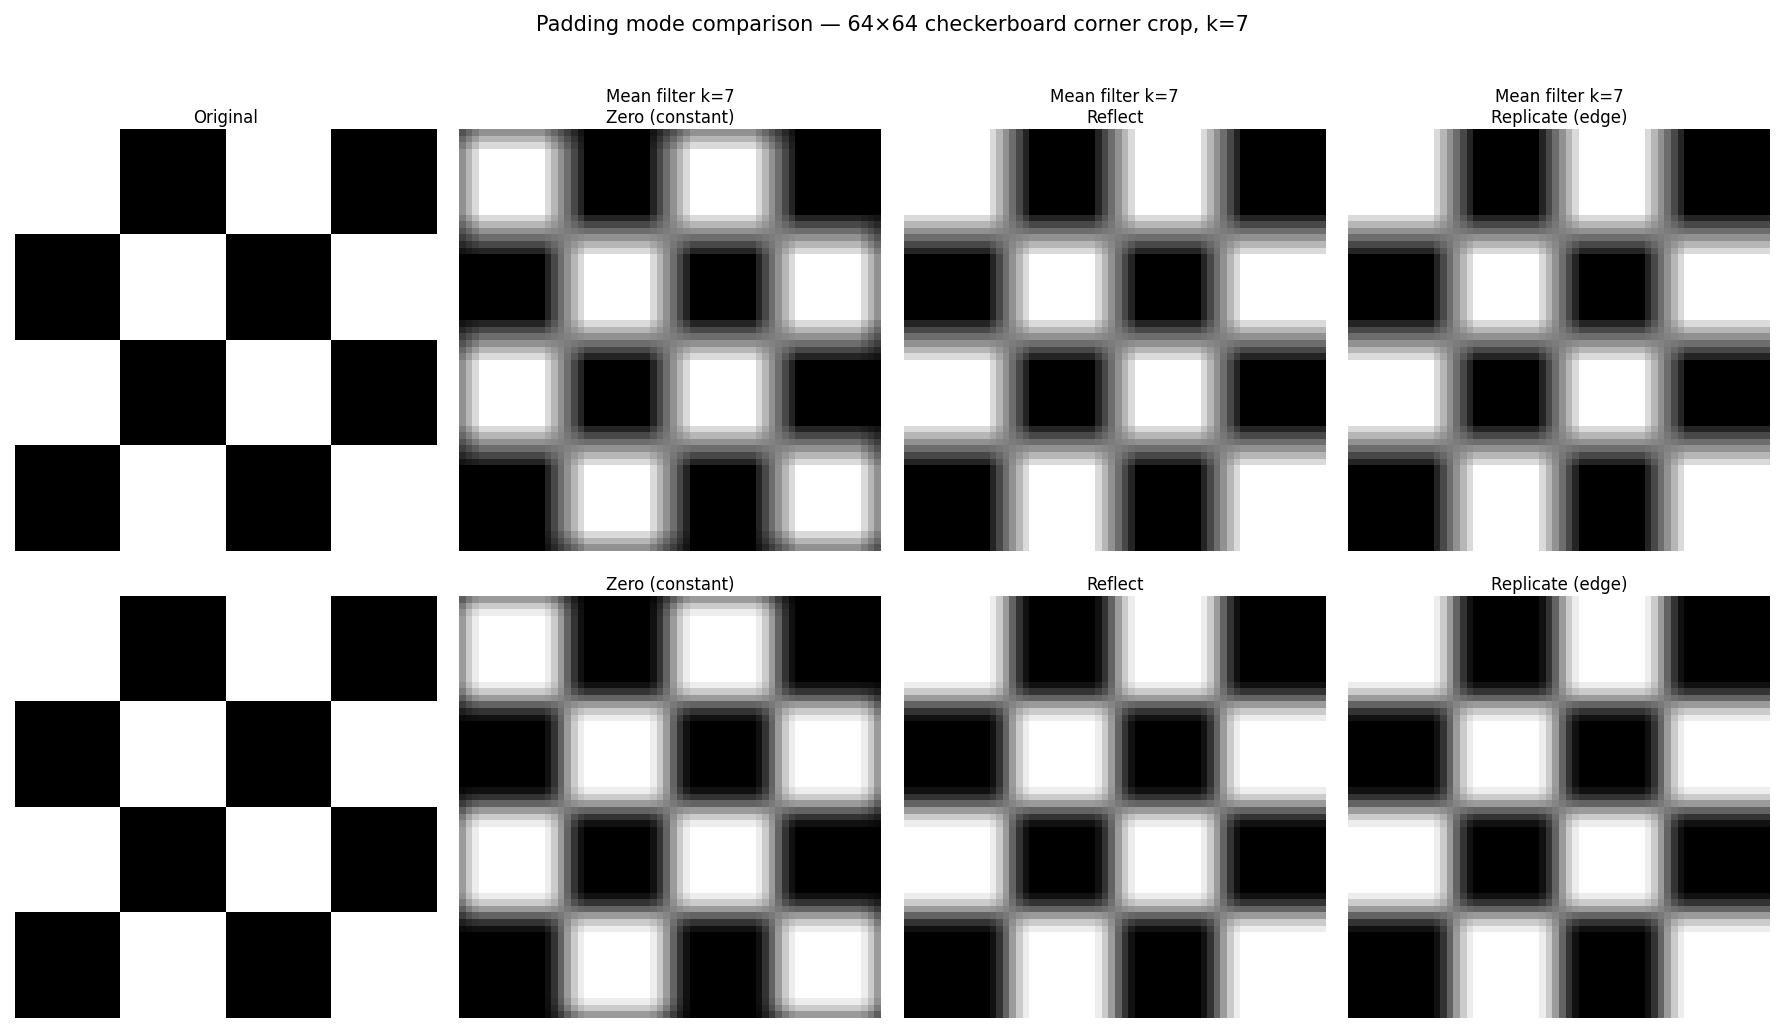
\includegraphics[width=\linewidth]{padding_comparison}
  \caption{Padding mode comparison on a 64$\times$64 checkerboard corner crop.
           Top row: mean filter ($k=7$).
           Bottom row: Gaussian filter ($k=7$, $\sigma=2$).
           Left column: original crop.
           Subsequent columns: zero (constant), reflect, replicate padding.
           Zero padding produces a dark border artefact; reflect and replicate
           avoid it. Reflect is smoother; replicate has a sharper edge exactly
           at the image boundary.}
  \label{fig:padding}
\end{figure}

\subsection{Mean Filter}

The box (mean) filter replaces each pixel with the unweighted average of its
$k \times k$ neighbourhood:

\begin{equation}
  K_{\text{mean}}[m,n] = \frac{1}{k^2}, \quad 0 \le m,n < k.
\end{equation}

Mean filtering is the maximum-likelihood denoiser for additive Gaussian noise
under a flat (uniform) image prior; it is fast but blurs edges because it
weights all neighbours equally regardless of distance.
Figure~\ref{fig:mean} shows the effect at $k \in \{3, 7, 15\}$.

\subsection{Gaussian Filter}

The Gaussian kernel is the unique linear filter that is simultaneously
rotationally symmetric and separable.
I generate it analytically from

\begin{equation}
  G_\sigma(x, y) = \exp\!\left(-\frac{x^2 + y^2}{2\sigma^2}\right),
  \quad K_\sigma = \frac{G_\sigma}{\sum_{x,y} G_\sigma(x,y)},
  \label{eq:gaussian}
\end{equation}

where the normalisation ensures that a constant image is unchanged.
The grid is centred at zero: for a kernel of size $k$ the coordinates run from
$-\lfloor k/2 \rfloor$ to $\lfloor k/2 \rfloor$.
Figure~\ref{fig:gauss_kernels} visualises the kernels as heat maps.

Compared to the mean filter, Gaussian smoothing assigns exponentially less
weight to distant pixels: nearby pixels dominate, so fine structure at scales
$\ll \sigma$ is suppressed while large-scale structure is preserved.
The transition from noise-suppression to structural blurring is controlled by
$\sigma$ independently of $k$ (provided $k \gtrsim 6\sigma$).
Figure~\ref{fig:gaussian} shows results for $\sigma \in \{0.5, 1.0, 2.0\}$
and $k \in \{3, 7, 15\}$.

\subsection{Laplacian Filter}

The Laplacian $\nabla^2 I = \partial^2 I/\partial x^2 + \partial^2 I/\partial y^2$
is the isotropic second derivative; its zero-crossings mark edges.
I implement two discrete approximations:

\paragraph{4-connected (standard):}
\begin{equation}
  K_{\text{std}} =
  \begin{bmatrix} 0 & 1 & 0 \\ 1 & -4 & 1 \\ 0 & 1 & 0 \end{bmatrix}.
\end{equation}

\paragraph{8-connected (diagonal):}
\begin{equation}
  K_{\text{diag}} =
  \begin{bmatrix} 1 & 1 & 1 \\ 1 & -8 & 1 \\ 1 & 1 & 1 \end{bmatrix}.
\end{equation}

Both kernels sum to zero (a necessary condition for a derivative operator),
so they produce zero response in constant regions.
The diagonal variant weights the four diagonal neighbours equally to the
axis-aligned ones, making the approximation more isotropic.
Output values can be negative; all visualisations apply min-max normalisation
to $[0,255]$ before display.
Figure~\ref{fig:laplacian} compares both kernels on the three input types.

\subsection{Sobel Filter}

The Sobel operator estimates the first-order spatial gradient using
separable kernels that simultaneously smooth in the orthogonal direction
(reducing noise sensitivity) and differentiate in the target direction.

\paragraph{3$\times$3 kernels:}
\begin{equation}
  K_x =
  \begin{bmatrix} -1 & 0 & 1 \\ -2 & 0 & 2 \\ -1 & 0 & 1 \end{bmatrix},
  \quad
  K_y =
  \begin{bmatrix} -1 & -2 & -1 \\ 0 & 0 & 0 \\ 1 & 2 & 1 \end{bmatrix}.
\end{equation}

Each kernel is the outer product of the binomial smoothing vector
$\mathbf{s}_3 = [1,2,1]^\top$ and the central-difference vector
$\mathbf{d}_3 = [-1,0,1]^\top$:
$K_x = \mathbf{s}_3 \mathbf{d}_3^\top$,
$K_y = \mathbf{d}_3 \mathbf{s}_3^\top$.

\paragraph{5$\times$5 kernels:}
The same outer-product construction generalises using the next binomial row
$\mathbf{s}_5 = [1,4,6,4,1]^\top$ and the derivative vector
$\mathbf{d}_5 = [-1,-2,0,2,1]^\top$:

\begin{equation}
  K_x^{(5)} = \mathbf{s}_5 \mathbf{d}_5^\top, \quad
  K_y^{(5)} = \mathbf{d}_5 \mathbf{s}_5^\top.
  \label{eq:sobel5}
\end{equation}

This is the exact construction used by OpenCV internally for
\texttt{cv2.Sobel(..., ksize=5)}.

Gradient magnitude and direction are computed as
\begin{equation}
  M = \sqrt{G_x^2 + G_y^2}, \quad
  \theta = \operatorname{atan2}(G_y, G_x) \in [-\pi, \pi].
  \label{eq:sobelmag}
\end{equation}

Figure~\ref{fig:sobel} shows $G_x$, $G_y$, $M$, and $\theta$ for all three
input images.

% ─────────────────────────────────────────────────────────────────────────────
\section{Part 1: Results}

\subsection{Gaussian Kernels}

\begin{figure}[H]
  \centering
  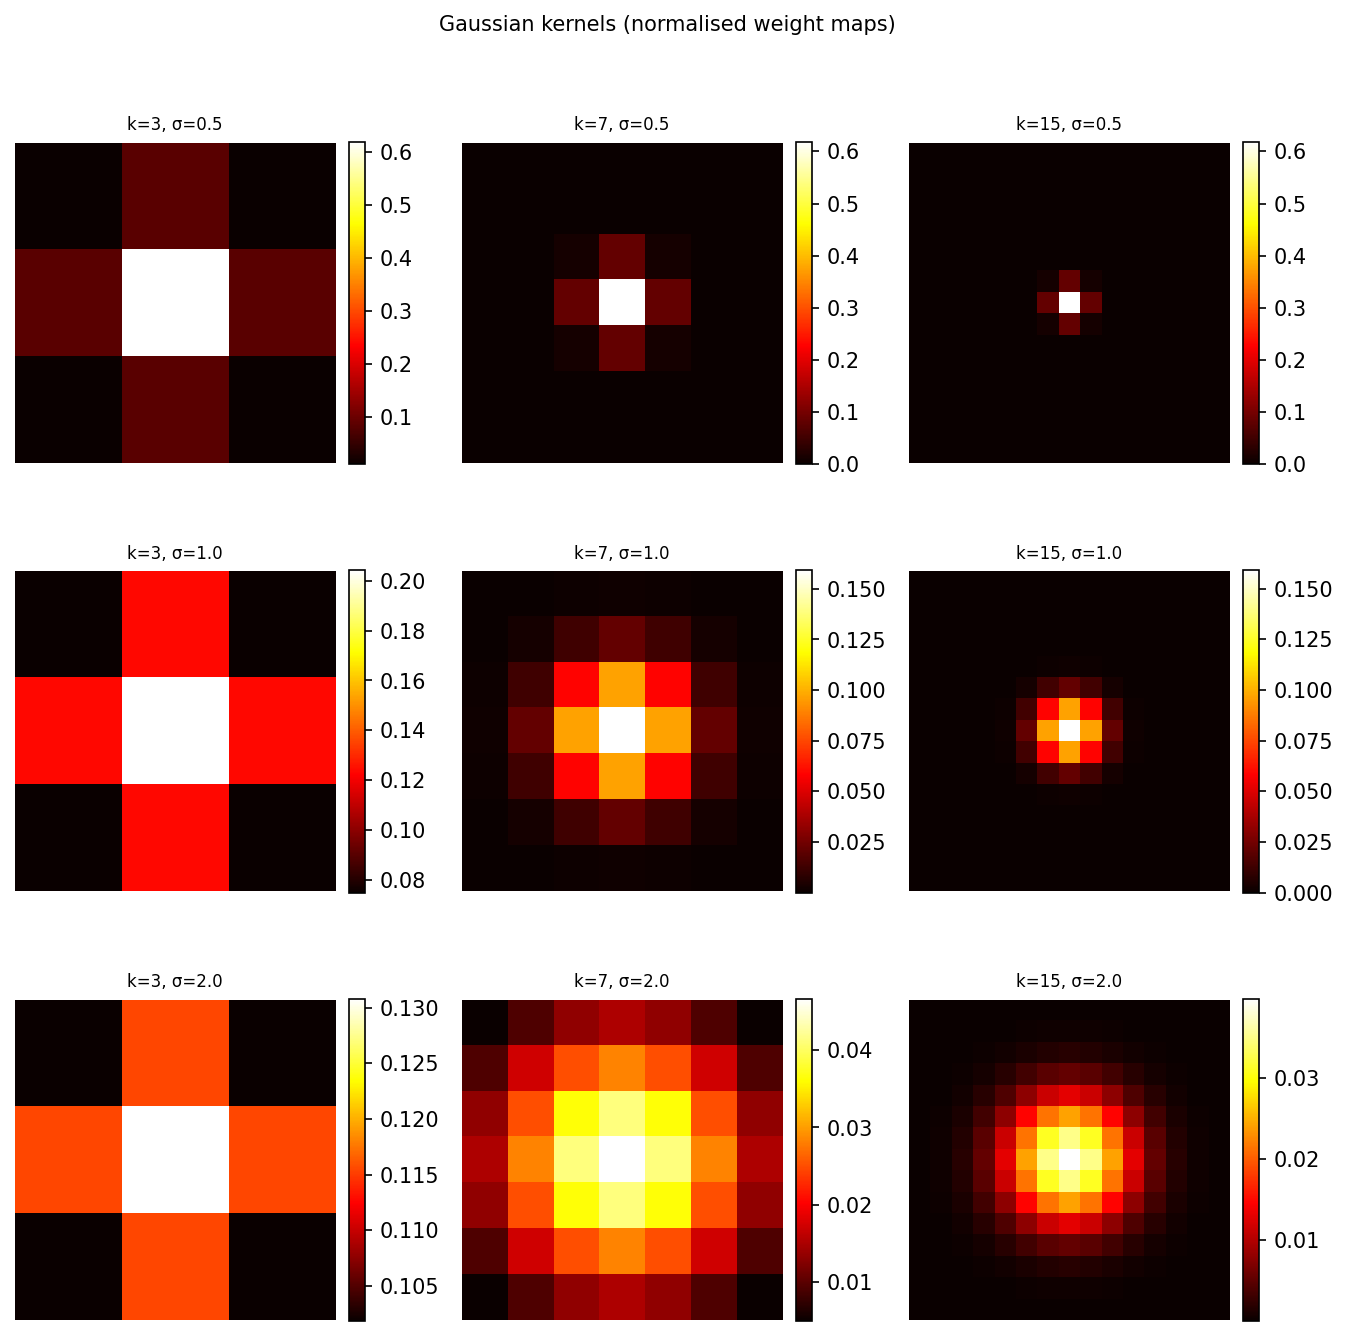
\includegraphics[width=\linewidth]{gaussian_kernels}
  \caption{Gaussian kernel weight maps for $\sigma \in \{0.5,1.0,2.0\}$
           (rows) and $k \in \{3,7,15\}$ (columns).
           At $\sigma=0.5, k=3$ nearly all weight concentrates in the centre
           pixel; at $\sigma=2.0, k=15$ the distribution approaches uniform.}
  \label{fig:gauss_kernels}
\end{figure}

\subsection{Mean Filter}

\begin{figure}[H]
  \centering
  \begin{subfigure}[b]{\linewidth}
    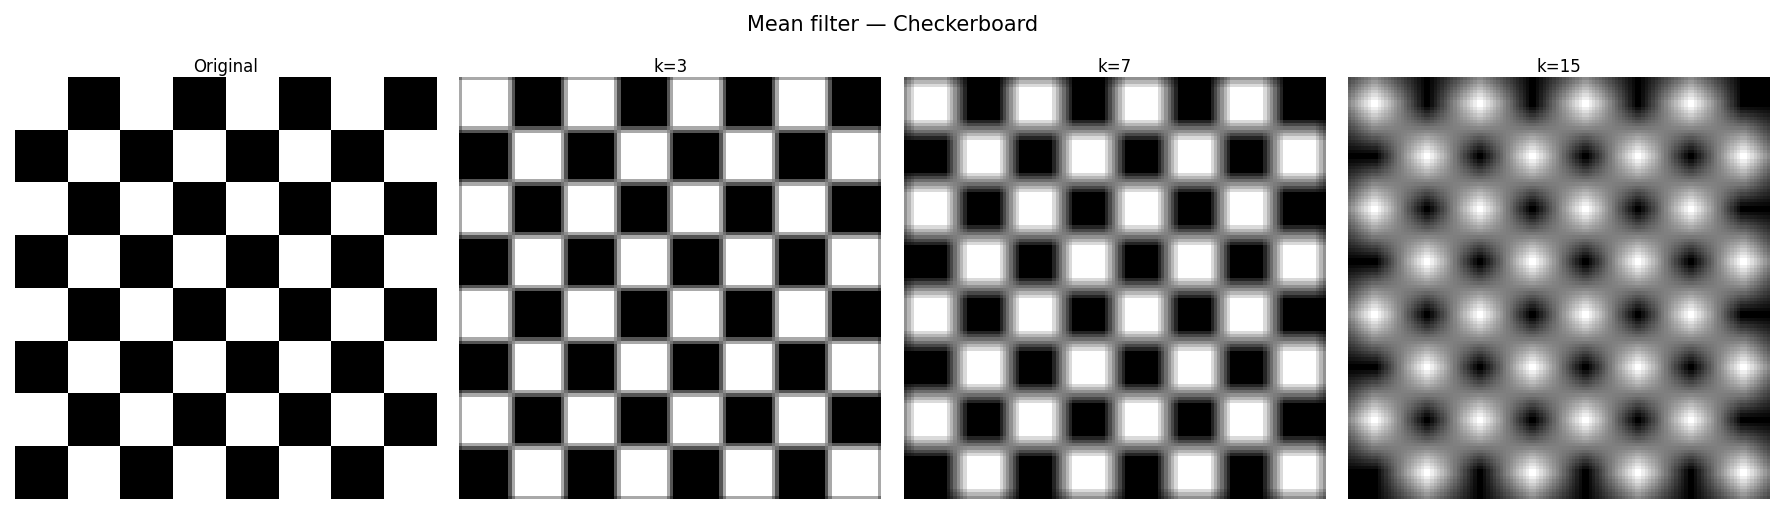
\includegraphics[width=\linewidth]{checkerboard_mean}
    \caption{Checkerboard input.}
  \end{subfigure}
  \begin{subfigure}[b]{\linewidth}
    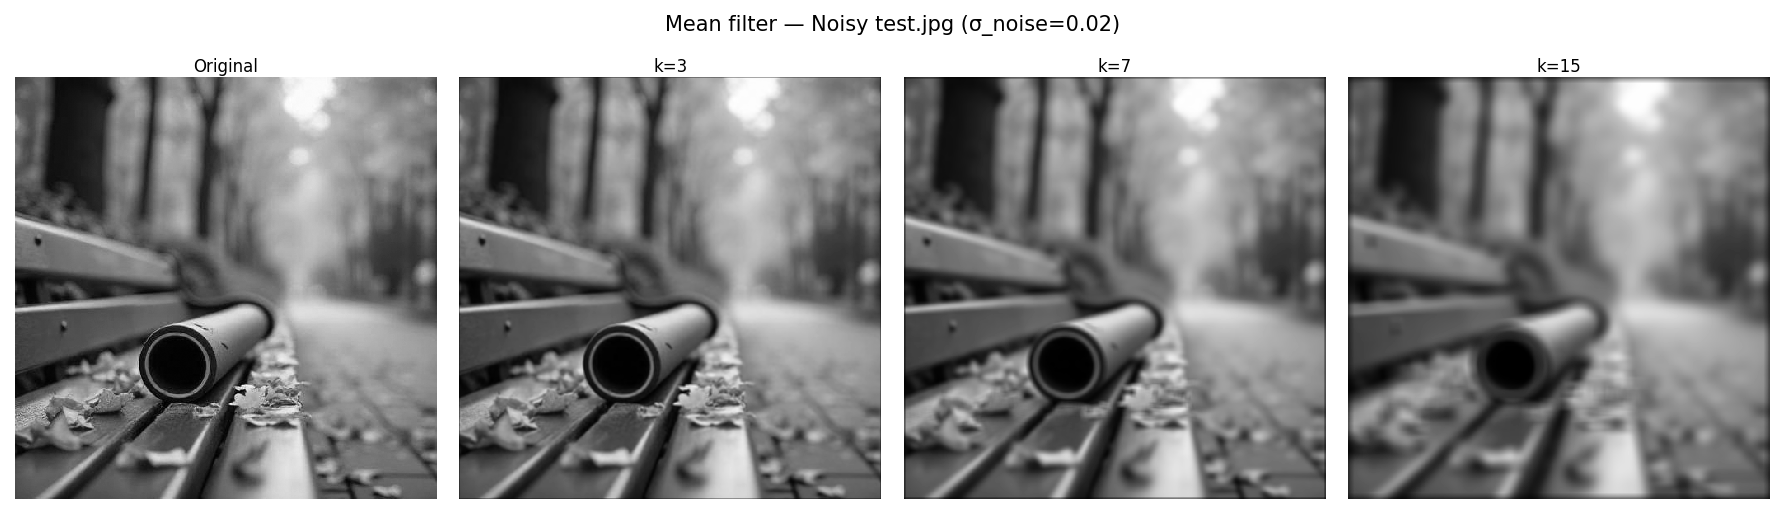
\includegraphics[width=\linewidth]{noisy_mean}
    \caption{Noisy test image.}
  \end{subfigure}
  \begin{subfigure}[b]{\linewidth}
    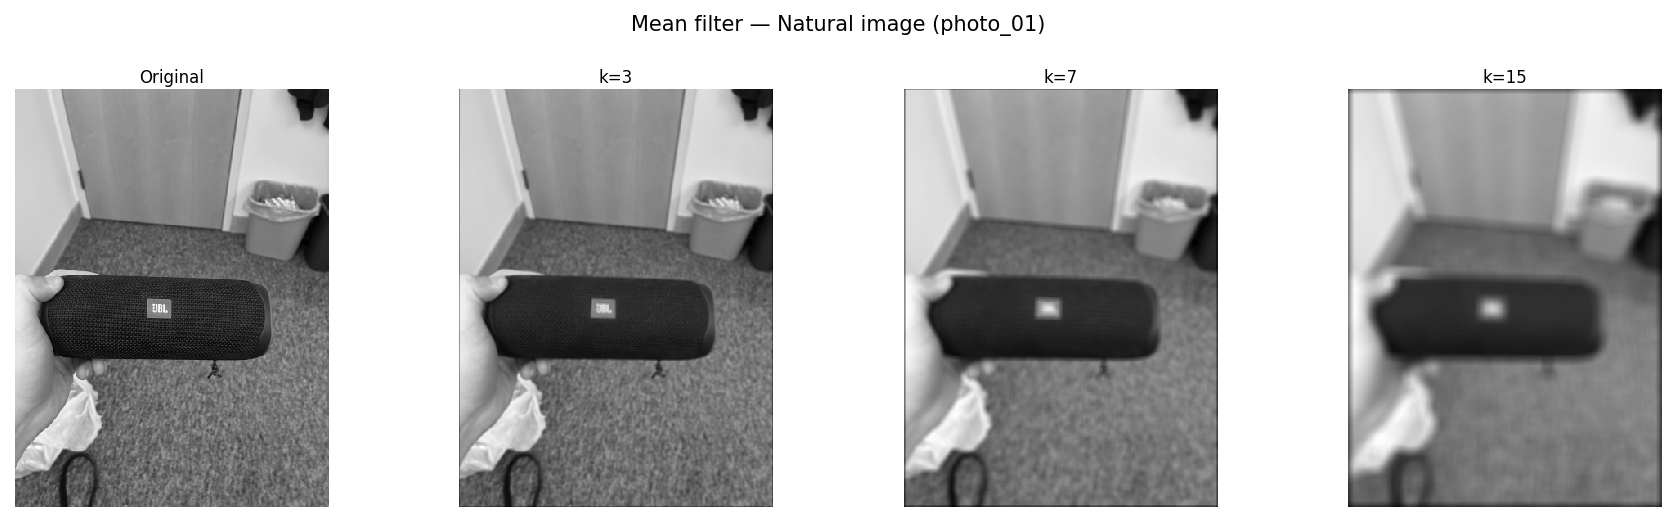
\includegraphics[width=\linewidth]{natural_mean}
    \caption{Natural image (photo\_01).}
  \end{subfigure}
  \caption{Mean filter at $k \in \{3, 7, 15\}$.
           Larger kernels progressively blur edges; the checkerboard shows
           pronounced ringing artefacts at $k=15$ because the box kernel has
           large Gibbs lobes in the frequency domain.}
  \label{fig:mean}
\end{figure}

\subsection{Gaussian Filter}

\begin{figure}[p]
  \centering
  \begin{subfigure}[b]{0.95\linewidth}
    \vspace{-0.5em}
    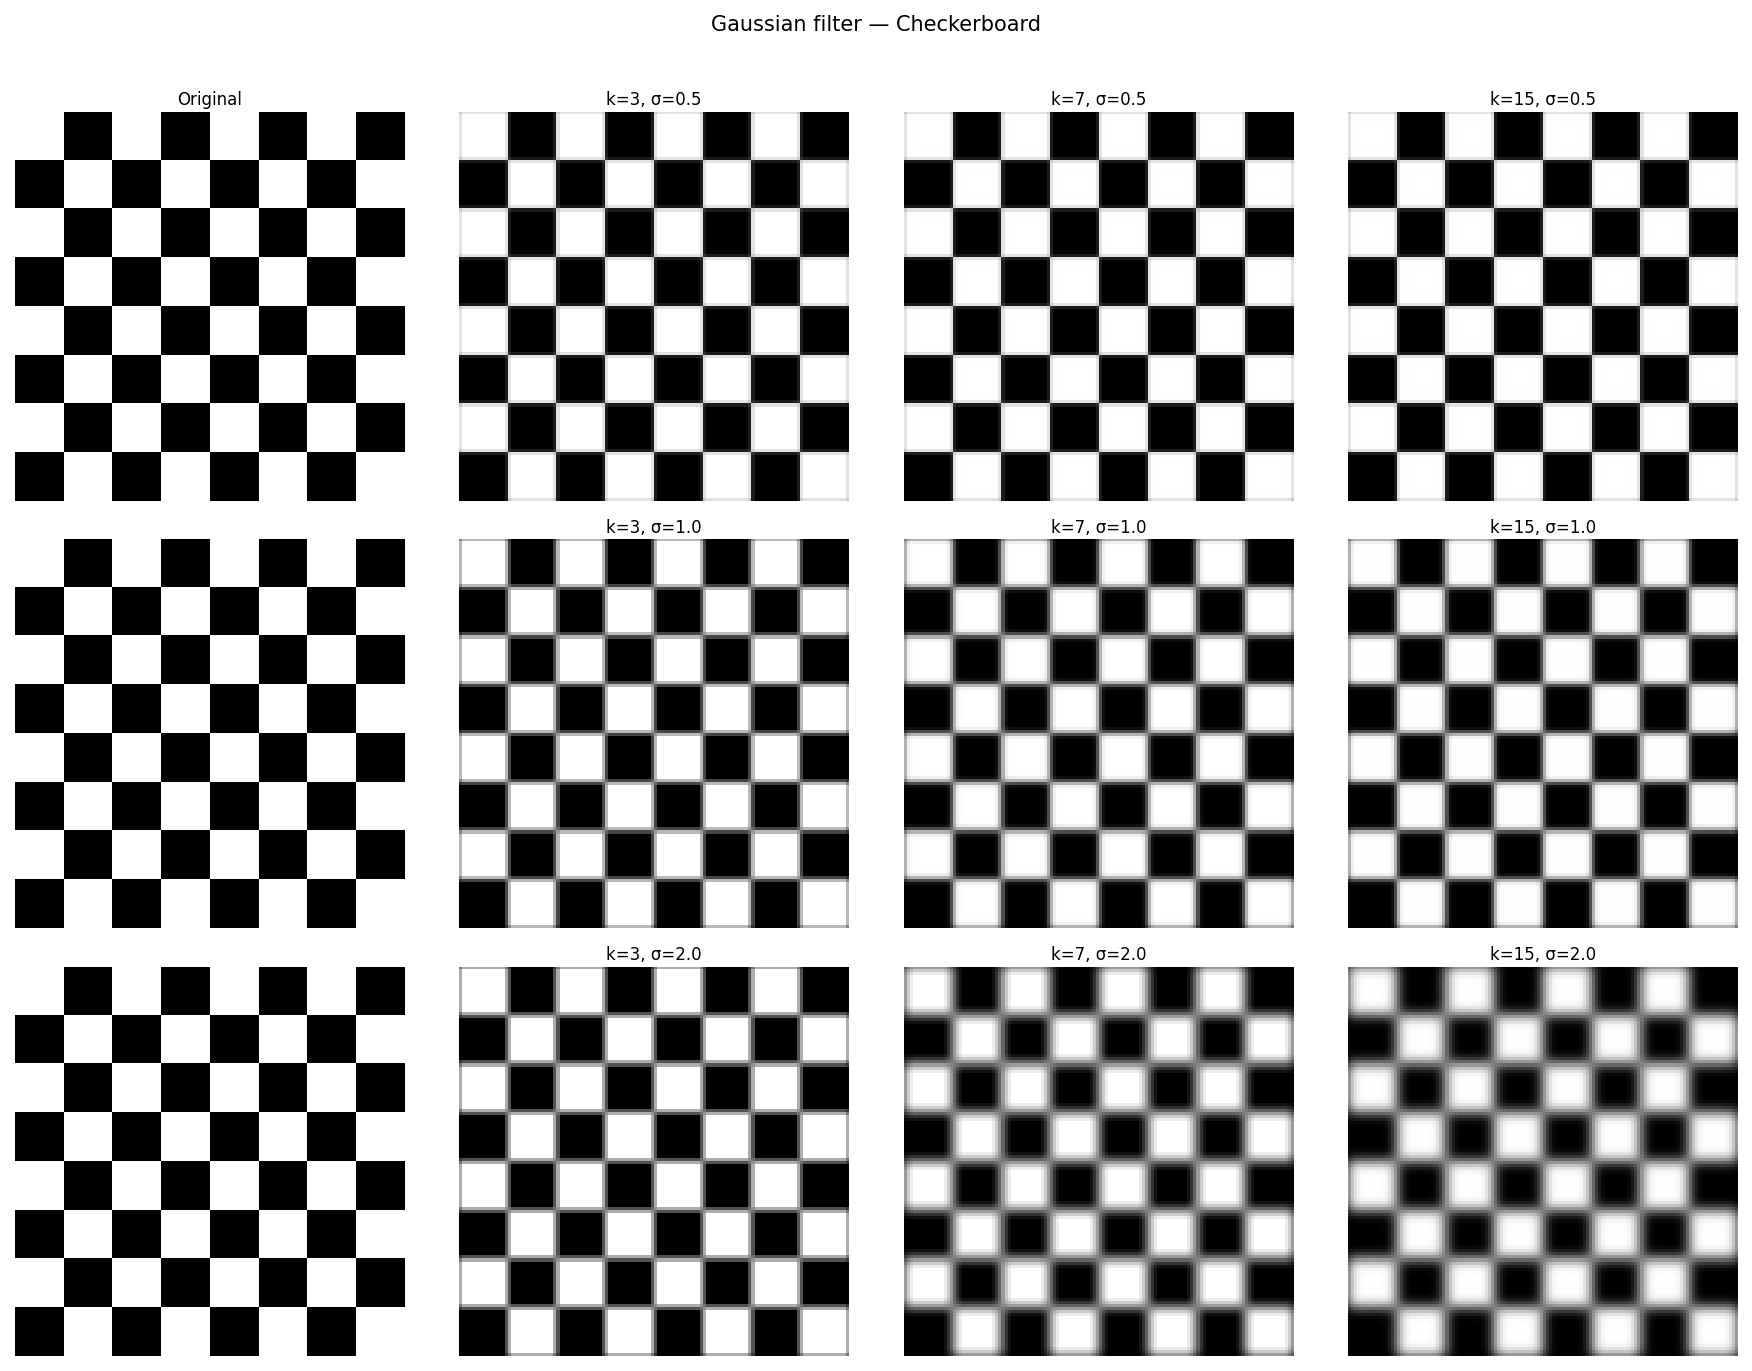
\includegraphics[width=\linewidth]{checkerboard_gaussian}
    \caption{Checkerboard: sigma varies across rows, kernel size across columns.}
  \end{subfigure}\\[0.3em]
  \begin{subfigure}[b]{0.95\linewidth}
    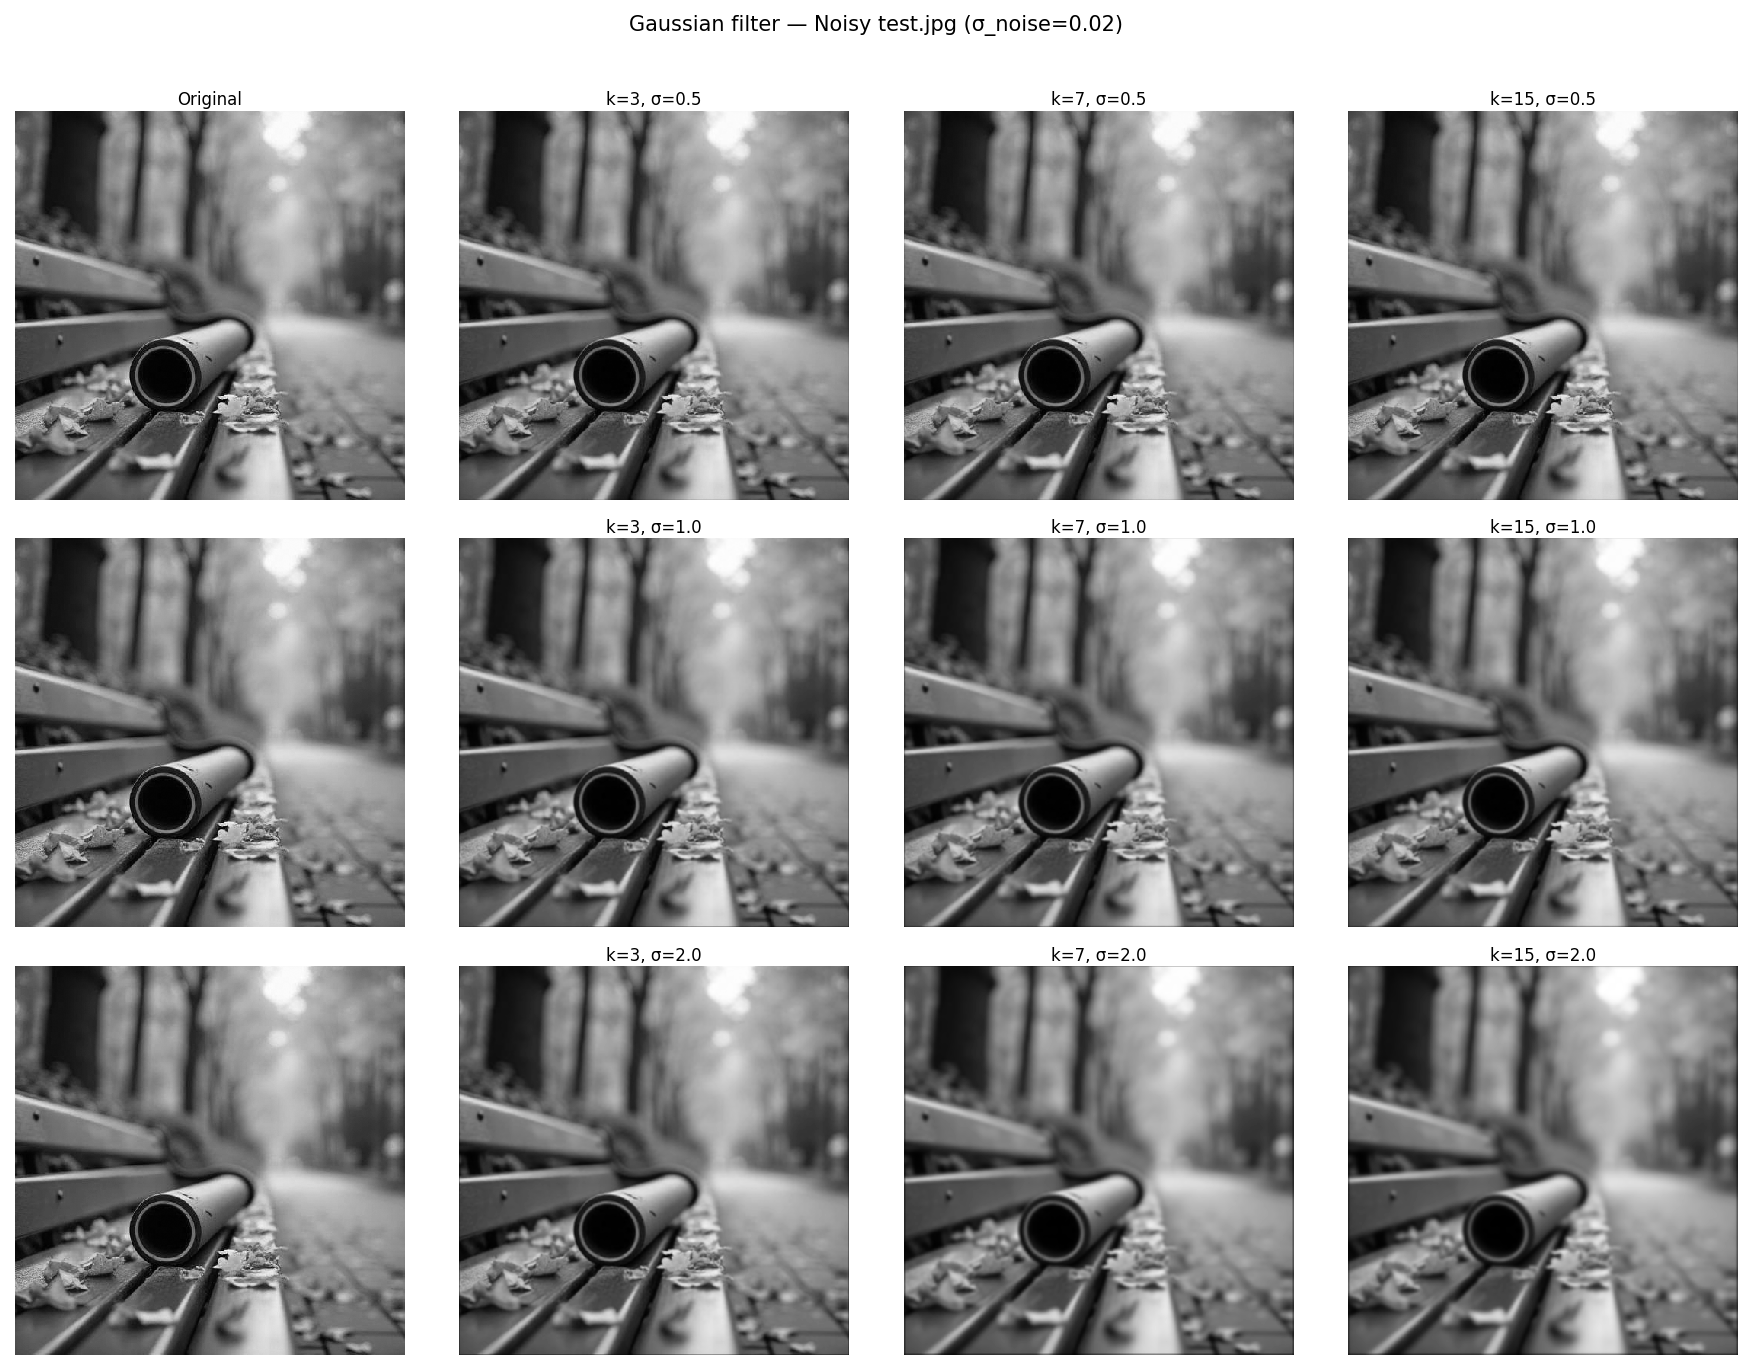
\includegraphics[width=\linewidth]{noisy_gaussian}
    \caption{Noisy test image.}
  \end{subfigure}\\[0.3em]
  \begin{subfigure}[b]{0.95\linewidth}
    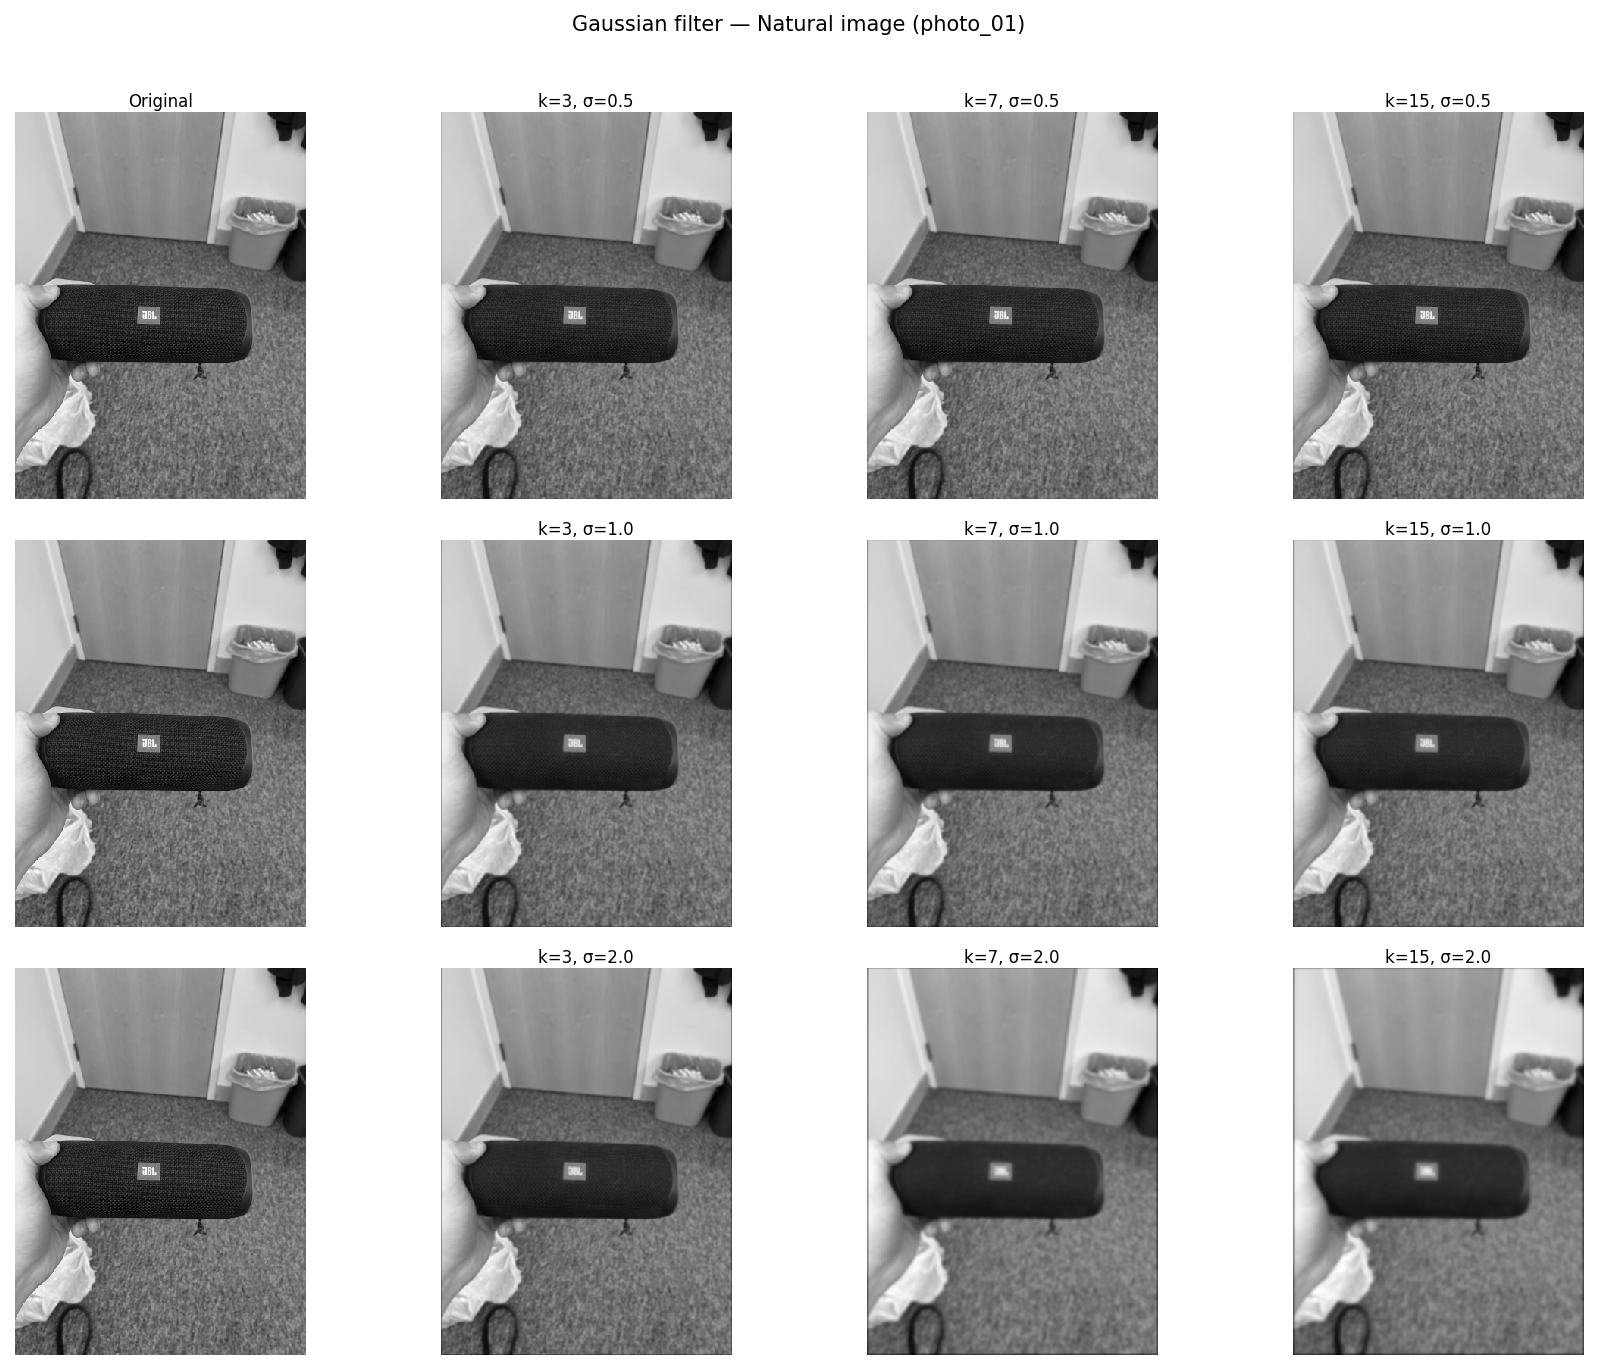
\includegraphics[width=\linewidth]{natural_gaussian}
    \caption{Natural image.}
  \end{subfigure}
  \caption{Gaussian filter for $\sigma \in \{0.5, 1.0, 2.0\}$ (rows) and
           $k \in \{3, 7, 15\}$ (columns).
           For a fixed $\sigma$, increasing $k$ beyond $6\sigma$ has negligible
           effect because the kernel tails are already vanishingly small.
           For a fixed $k$, increasing $\sigma$ progressively blurs the image.}
  \label{fig:gaussian}
\end{figure}

\subsection{Laplacian Filter}

\begin{figure}[H]
  \centering
  \begin{subfigure}[b]{\linewidth}
    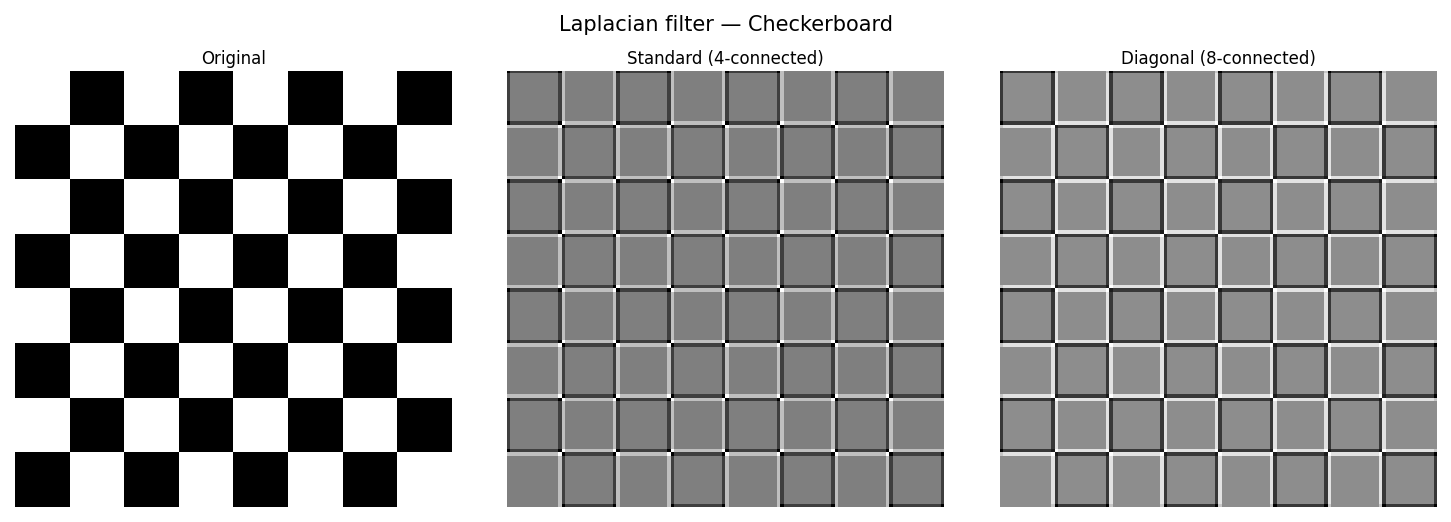
\includegraphics[width=\linewidth]{checkerboard_laplacian}
    \caption{Checkerboard.}
  \end{subfigure}
  \begin{subfigure}[b]{\linewidth}
    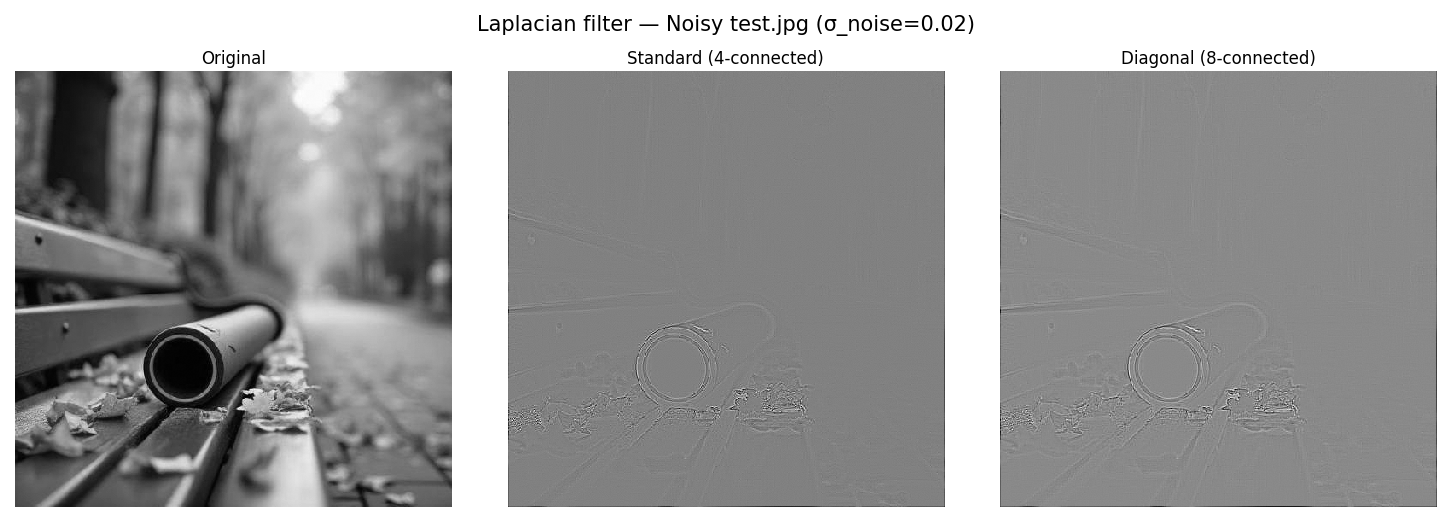
\includegraphics[width=\linewidth]{noisy_laplacian}
    \caption{Noisy test image.}
  \end{subfigure}
  \begin{subfigure}[b]{\linewidth}
    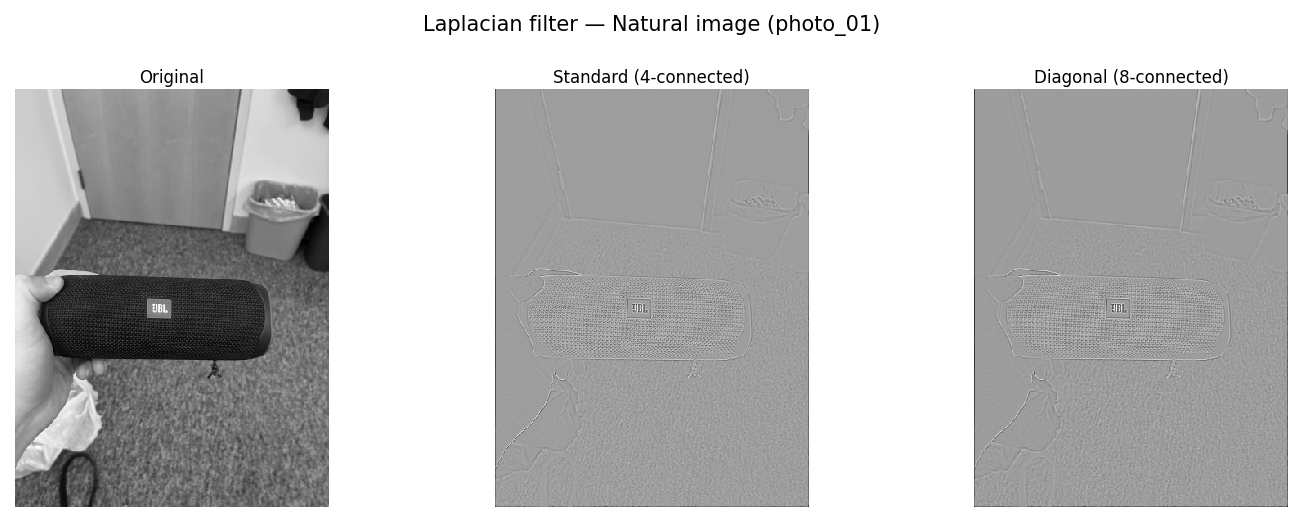
\includegraphics[width=\linewidth]{natural_laplacian}
    \caption{Natural image.}
  \end{subfigure}
  \caption{Laplacian filter with standard (4-connected) and diagonal
           (8-connected) kernels.
           The diagonal kernel detects edges at 45° angles that the standard
           kernel suppresses; this is visible on the checkerboard corners.
           The Laplacian is highly sensitive to noise---the noisy input produces
           a response dominated by per-pixel noise rather than image edges.}
  \label{fig:laplacian}
\end{figure}

\subsection{Sobel Filter}

\begin{figure}[H]
  \centering
  \begin{subfigure}[b]{\linewidth}
    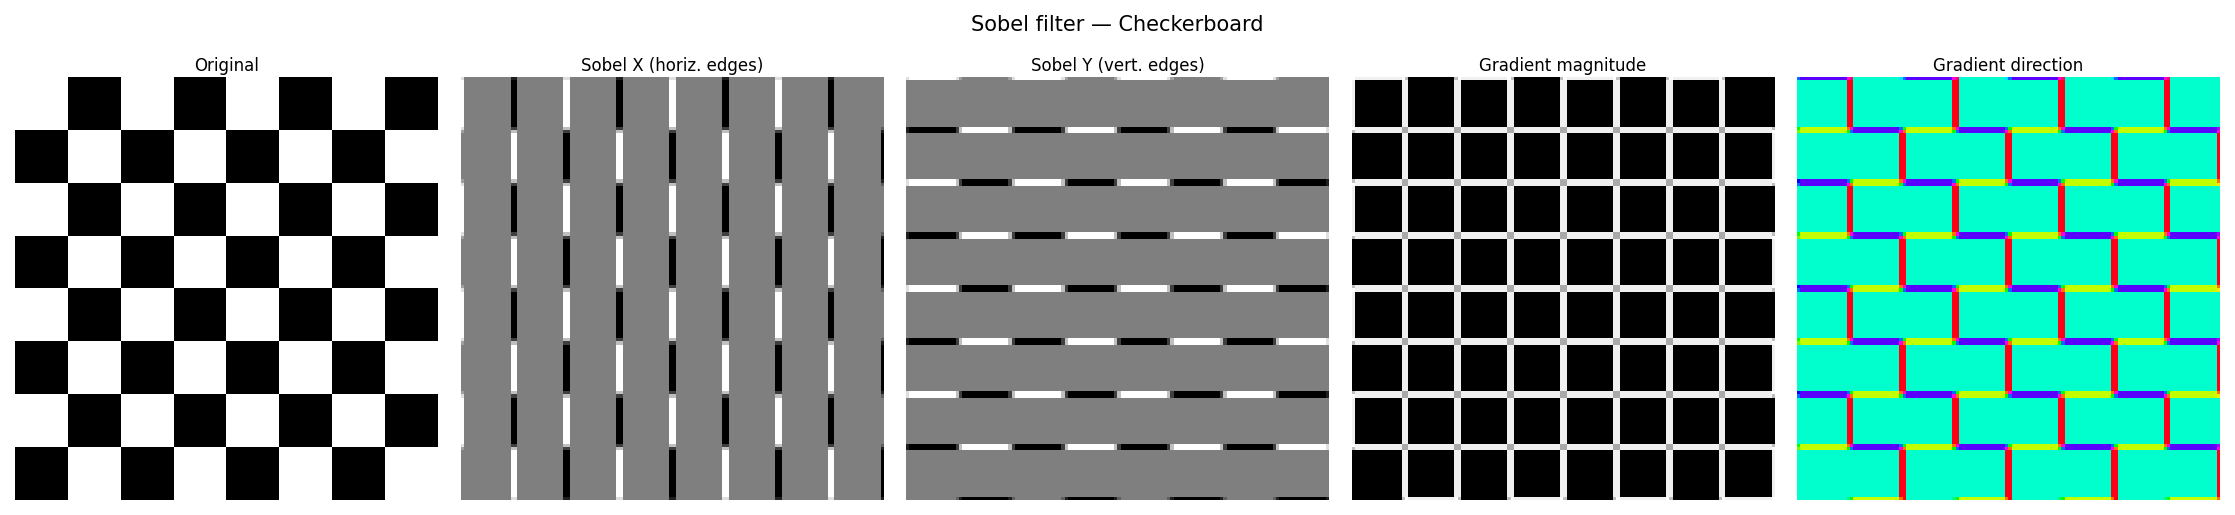
\includegraphics[width=\linewidth]{checkerboard_sobel}
    \caption{Checkerboard.}
  \end{subfigure}
  \begin{subfigure}[b]{\linewidth}
    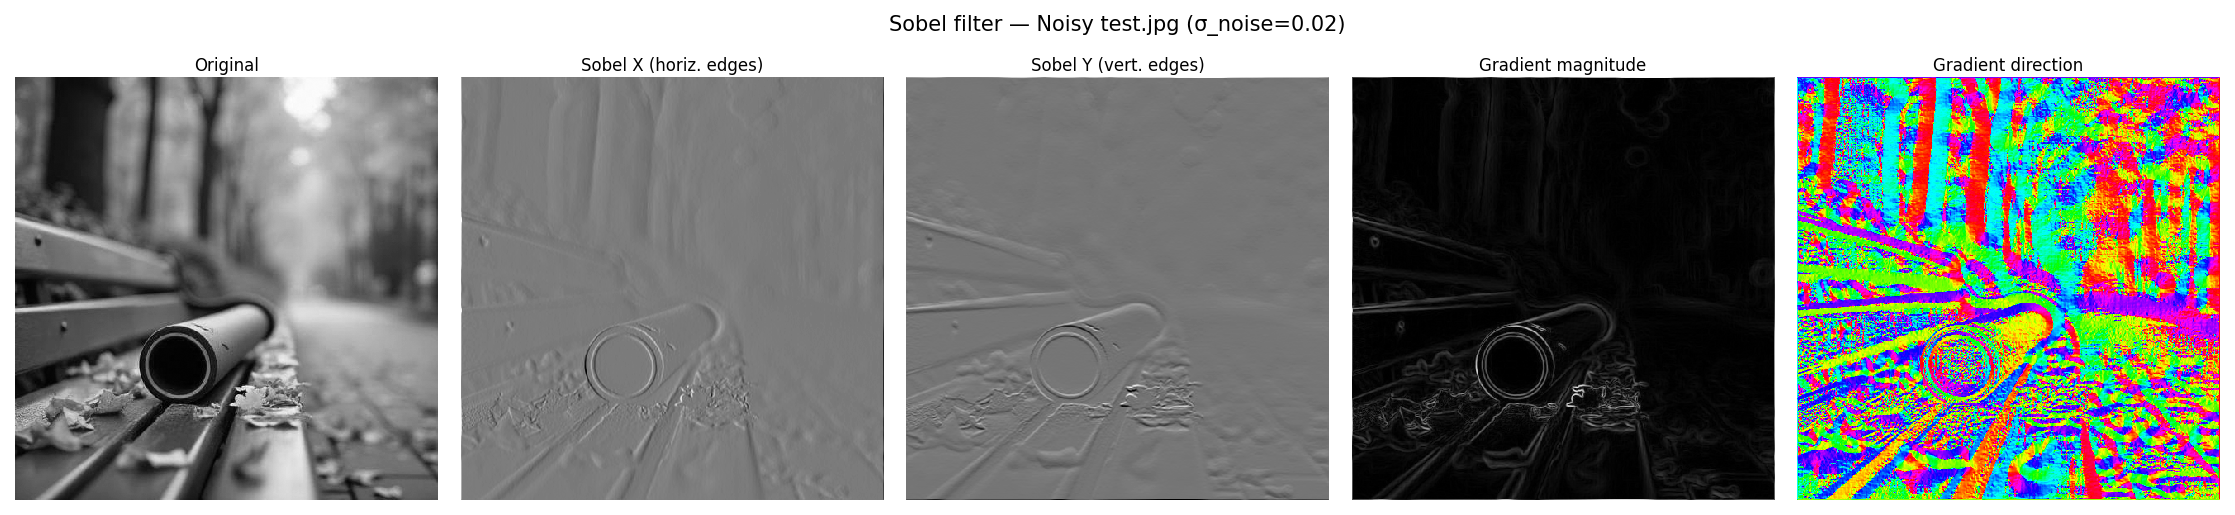
\includegraphics[width=\linewidth]{noisy_sobel}
    \caption{Gaussian-noisy test image.}
  \end{subfigure}
  \begin{subfigure}[b]{\linewidth}
    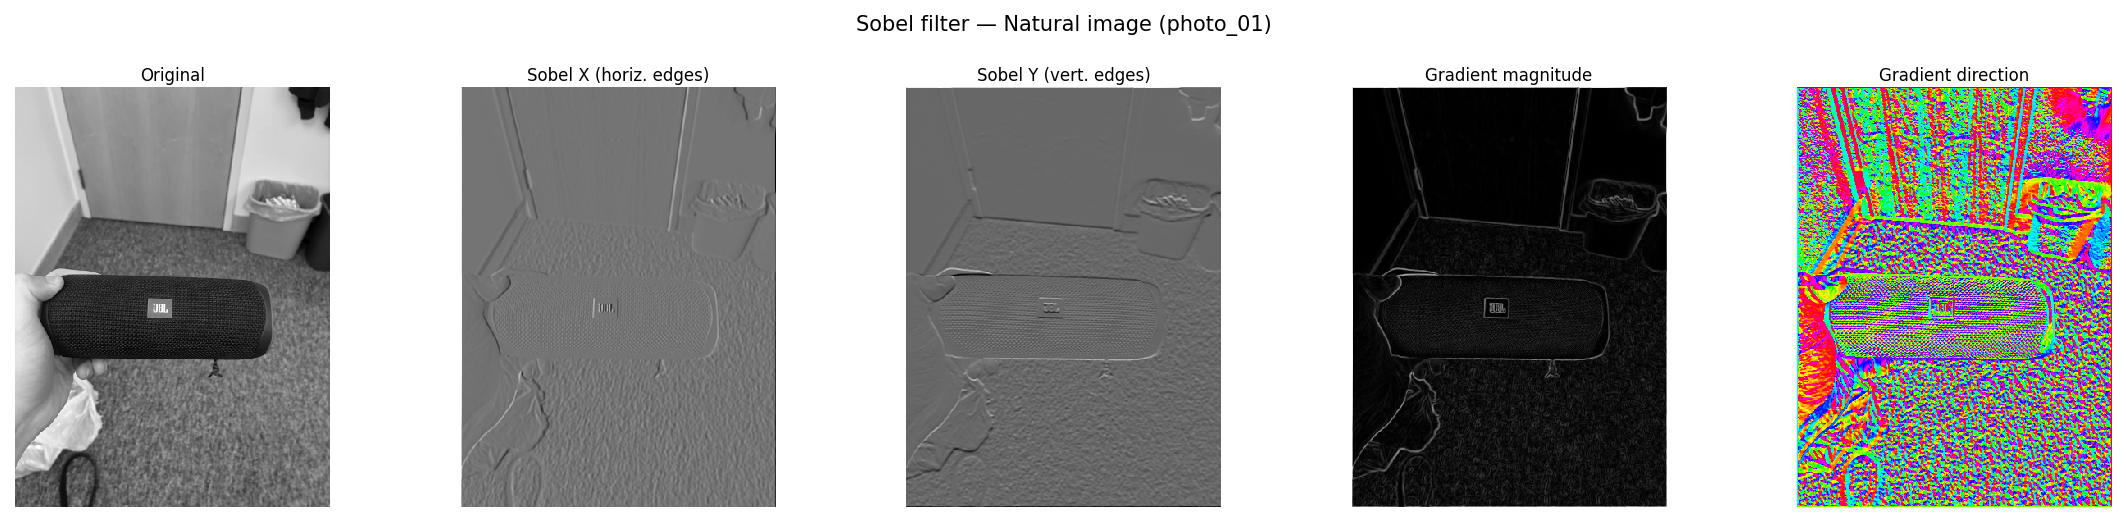
\includegraphics[width=\linewidth]{natural_sobel}
    \caption{Natural image.}
  \end{subfigure}
  \caption{Sobel $G_x$, $G_y$, magnitude $M$, and direction $\theta$
           (displayed with the HSV colormap so that $-\pi$ and $+\pi$ map to
           the same hue).
           The checkerboard shows clean axis-aligned gradients; the natural
           image shows strong responses at object boundaries.}
  \label{fig:sobel}
\end{figure}

\subsection{Salt-and-Pepper Noise}

\begin{figure}[H]
  \centering
  \begin{subfigure}[b]{\linewidth}
    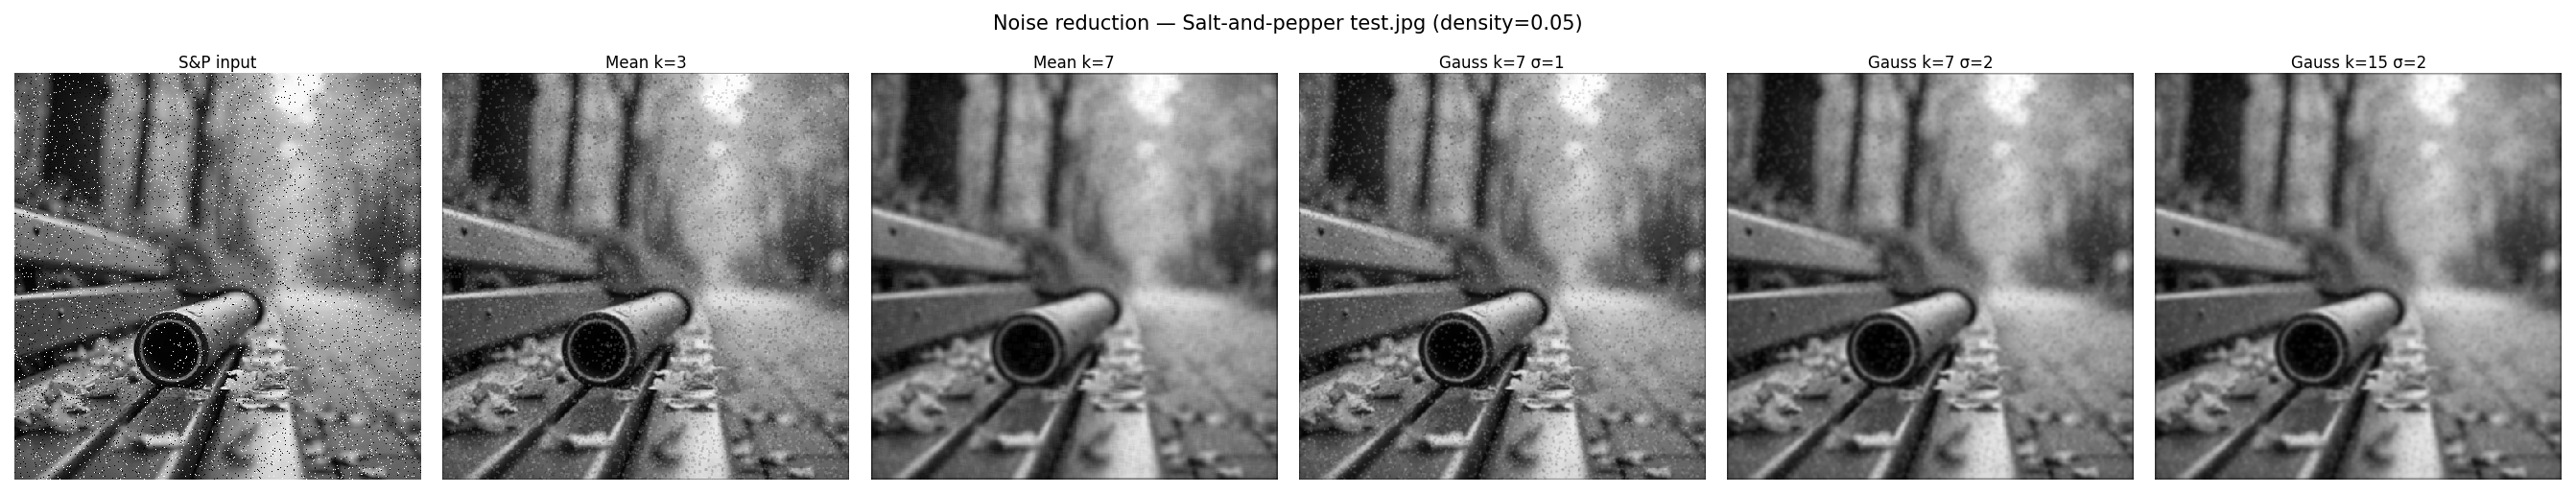
\includegraphics[width=\linewidth]{saltpepper_denoise}
    \caption{Mean and Gaussian filtering of salt-and-pepper noise (density 0.05).}
  \end{subfigure}
  \begin{subfigure}[b]{\linewidth}
    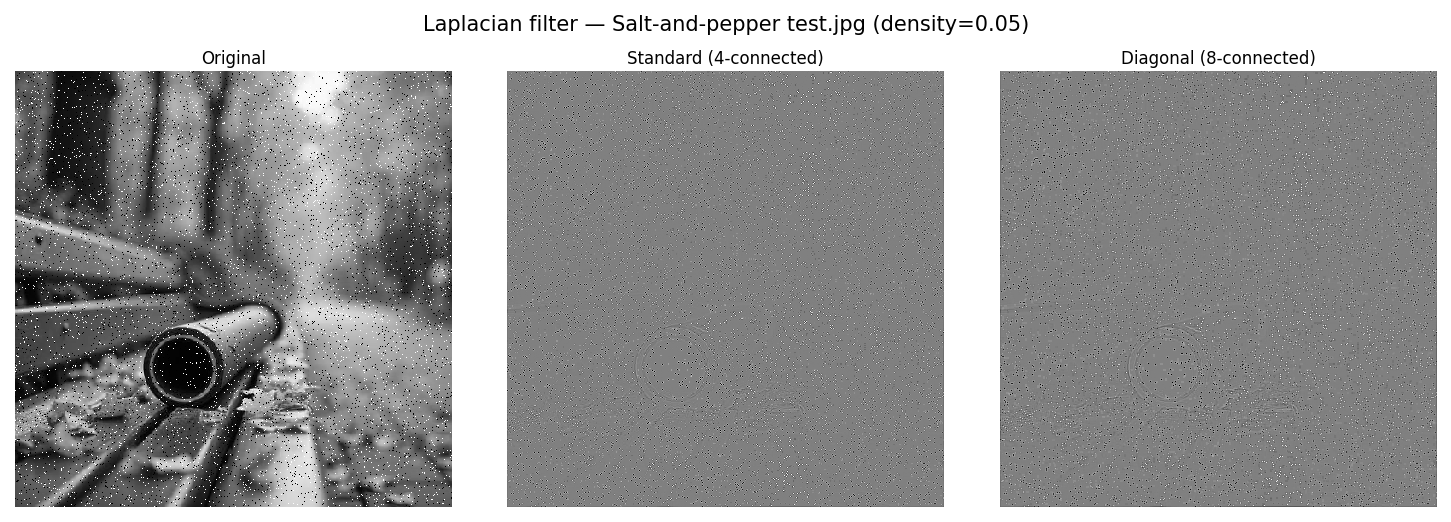
\includegraphics[width=\linewidth]{saltpepper_laplacian}
    \caption{Laplacian response on salt-and-pepper input.}
  \end{subfigure}
  \begin{subfigure}[b]{\linewidth}
    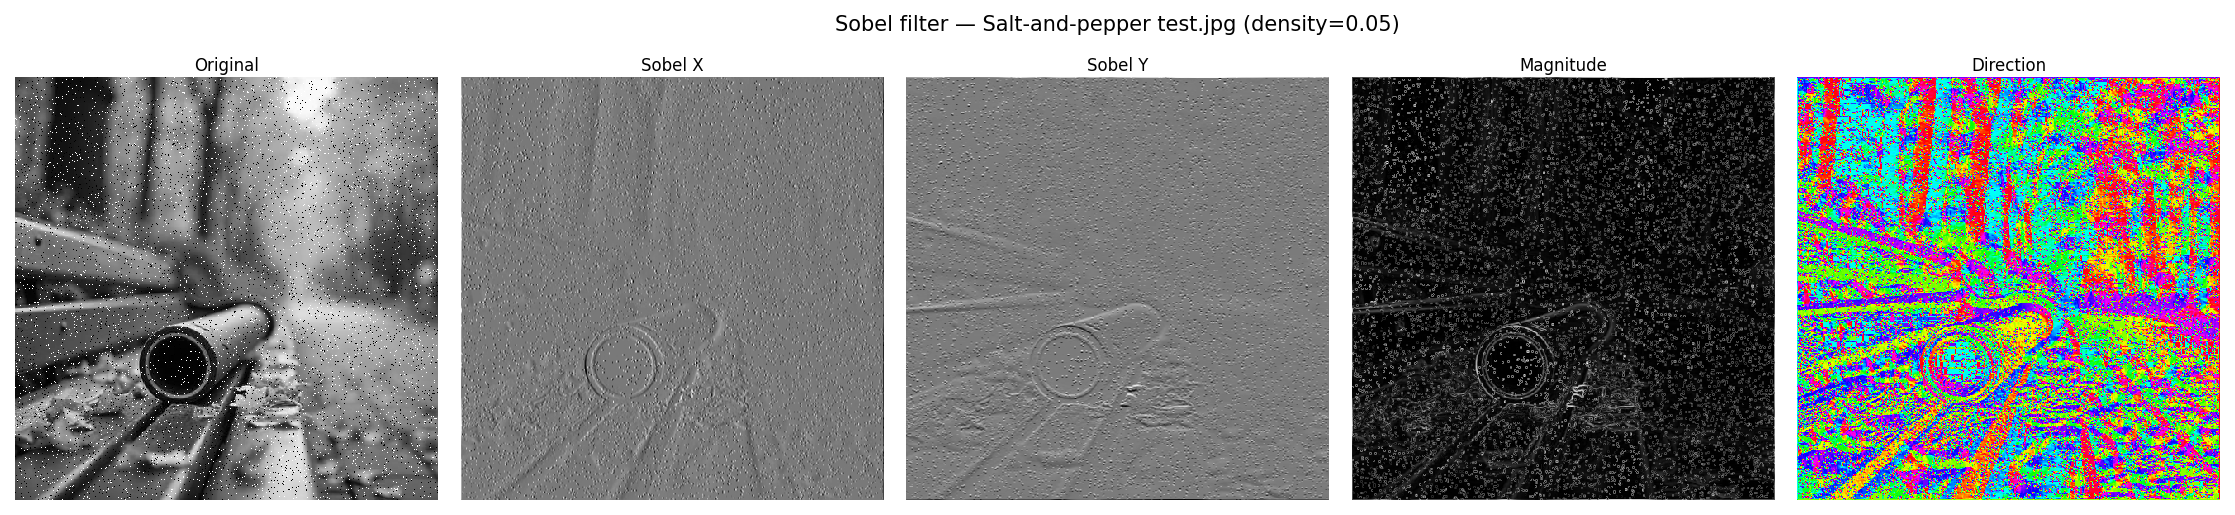
\includegraphics[width=\linewidth]{saltpepper_sobel}
    \caption{Sobel response on salt-and-pepper input.}
  \end{subfigure}
  \caption{Salt-and-pepper noise (density $= 0.05$) and filter responses.
           Mean and Gaussian filters reduce the impulse noise, but neither
           eliminates it as effectively as a median filter would.
           The Laplacian and Sobel responses are dominated by the noise spikes
           rather than image structure, demonstrating that first- and
           second-derivative filters require pre-smoothing before edge
           detection on impulsively noisy images.}
  \label{fig:saltpepper}
\end{figure}

\subsection{Personal Photo (Portrait)}

\begin{figure}[p]
  \centering
  \begin{subfigure}[b]{0.95\linewidth}
    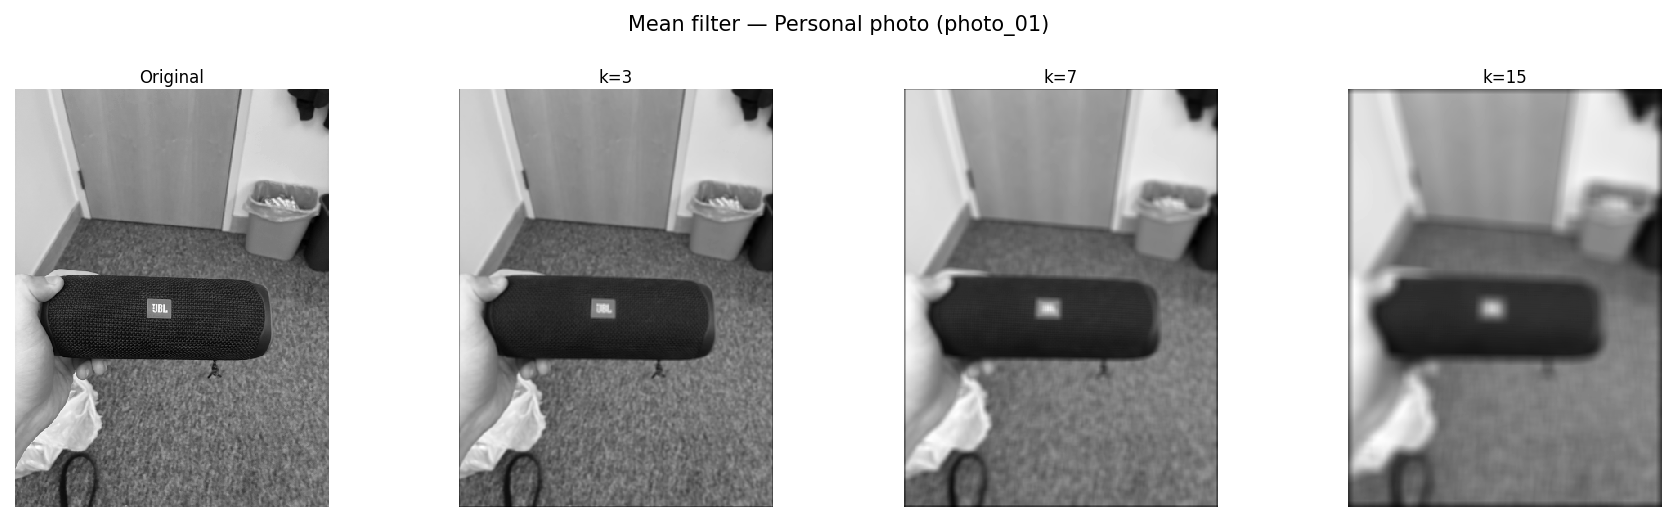
\includegraphics[width=\linewidth]{portrait_mean}
    \caption{Mean filter at $k \in \{3, 7, 15\}$.}
  \end{subfigure}\\[0.3em]
  \begin{subfigure}[b]{0.95\linewidth}
    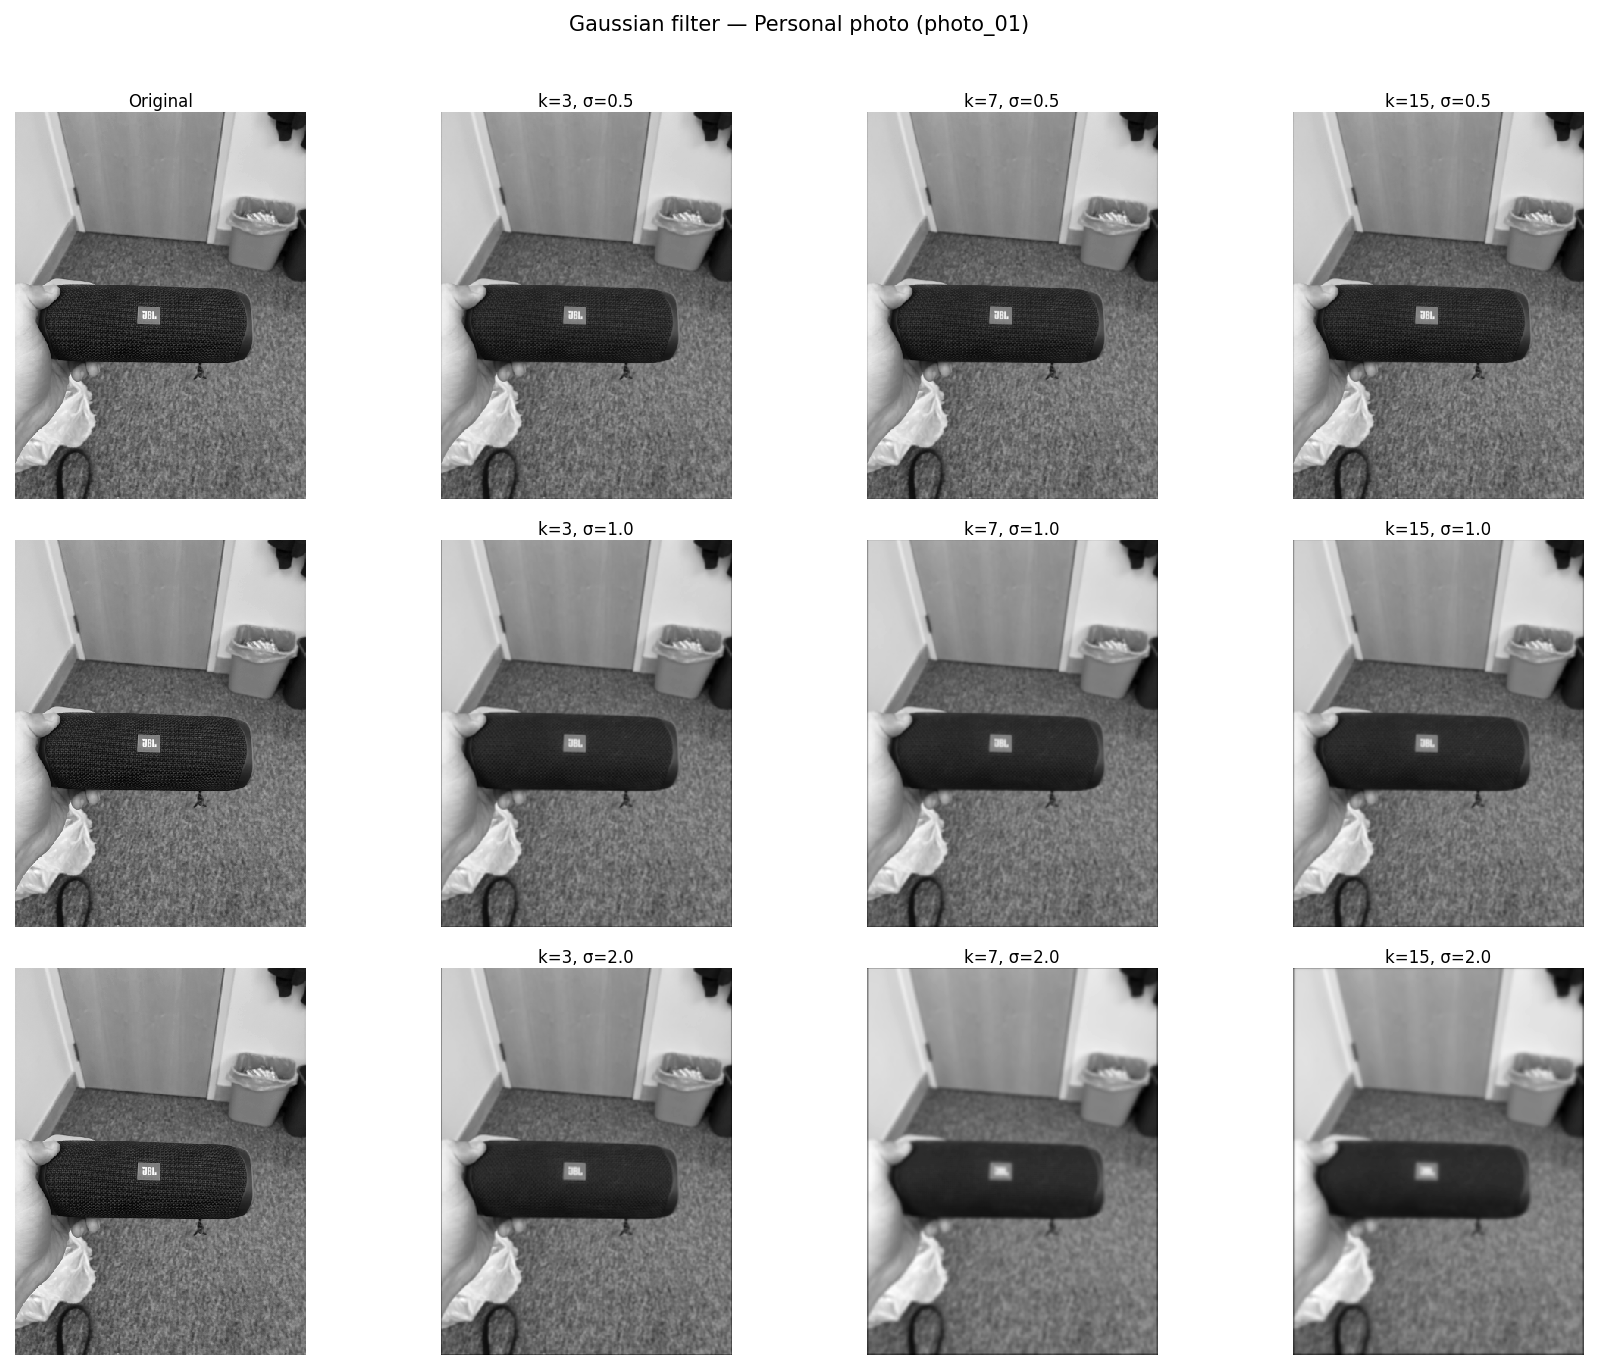
\includegraphics[width=\linewidth]{portrait_gaussian}
    \caption{Gaussian filter, $\sigma \in \{0.5,1.0,2.0\}$ (rows) $\times$ $k \in \{3,7,15\}$ (columns).}
  \end{subfigure}
  \caption{All Part~1 filters applied to a personally captured photograph
           (\texttt{photo\_01.jpg}, resized to 512\,px long edge) --- Part I.}
  \label{fig:portrait}
\end{figure}

\begin{figure}[p]
  \ContinuedFloat
  \centering
  \begin{subfigure}[b]{0.95\linewidth}
    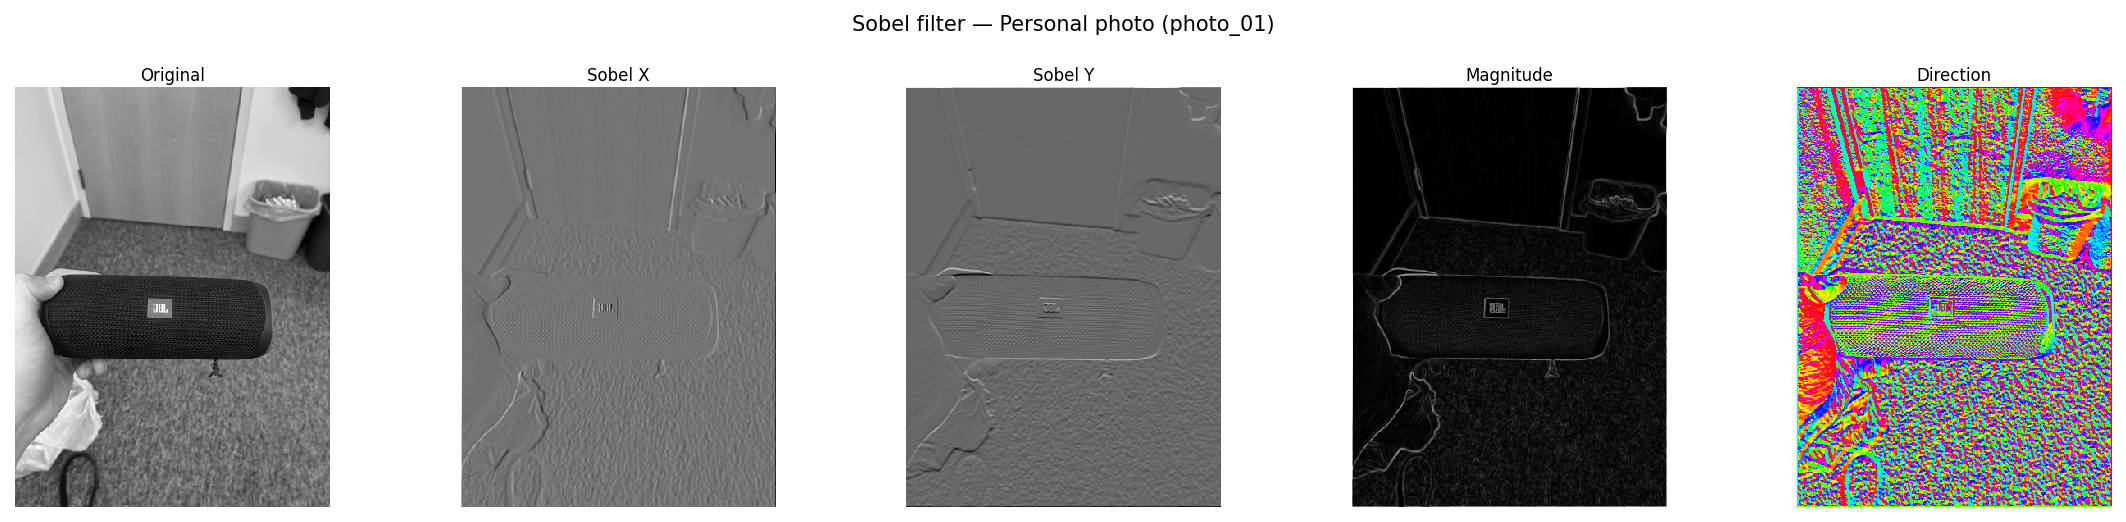
\includegraphics[width=\linewidth]{portrait_sobel}
    \caption{Sobel gradient components and magnitude.}
  \end{subfigure}\\[0.3em]
  \begin{subfigure}[b]{0.95\linewidth}
    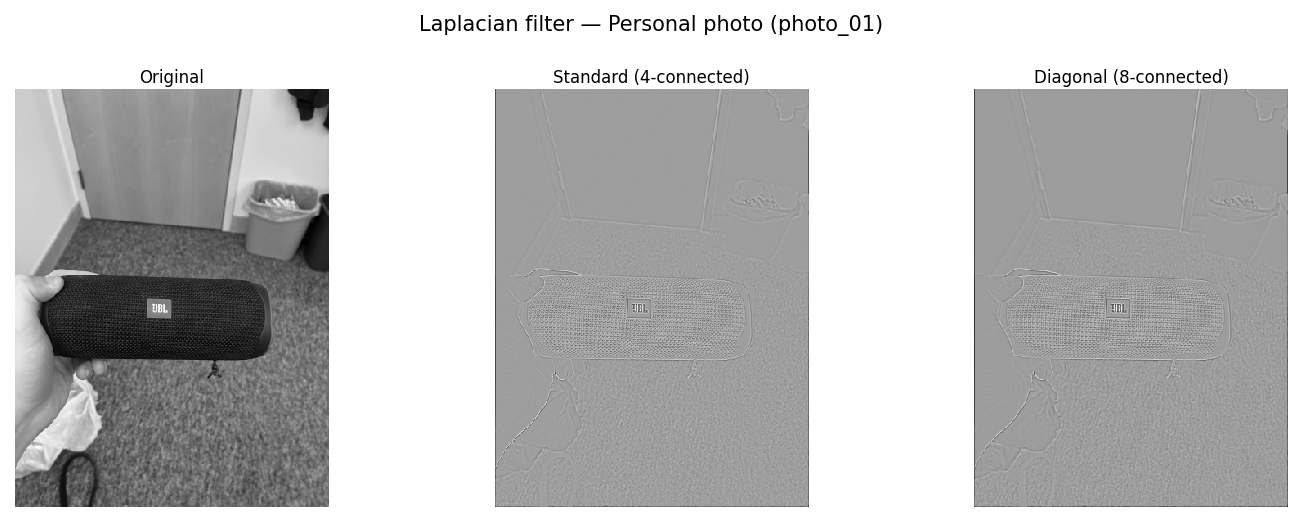
\includegraphics[width=\linewidth]{portrait_laplacian}
    \caption{Laplacian standard and diagonal kernels.}
  \end{subfigure}
  \caption{All Part~1 filters applied to a personally captured photograph --- Part II.
           The Sobel magnitude clearly outlines object boundaries and facial
           features in the image.
           Gaussian smoothing with $\sigma=2, k=15$ produces a painterly effect
           while preserving large-scale structure.}
\end{figure}

\subsection{OpenCV Comparison}

\begin{figure}[H]
  \centering
  \includegraphics[width=\linewidth]{test_opencv_comparison_smoothing}
  \caption{Smoothing filter comparison: OpenCV \texttt{cv2.blur} and
           \texttt{cv2.GaussianBlur} vs.\ my implementations at $k=5$.
           The outputs are visually indistinguishable; pixel-level differences
           are negligible (typically $< 1$ count on the uint8 scale), arising
           solely from floating-point accumulation order differences.}
  \label{fig:opencv_smooth}
\end{figure}

\begin{figure}[H]
  \centering
  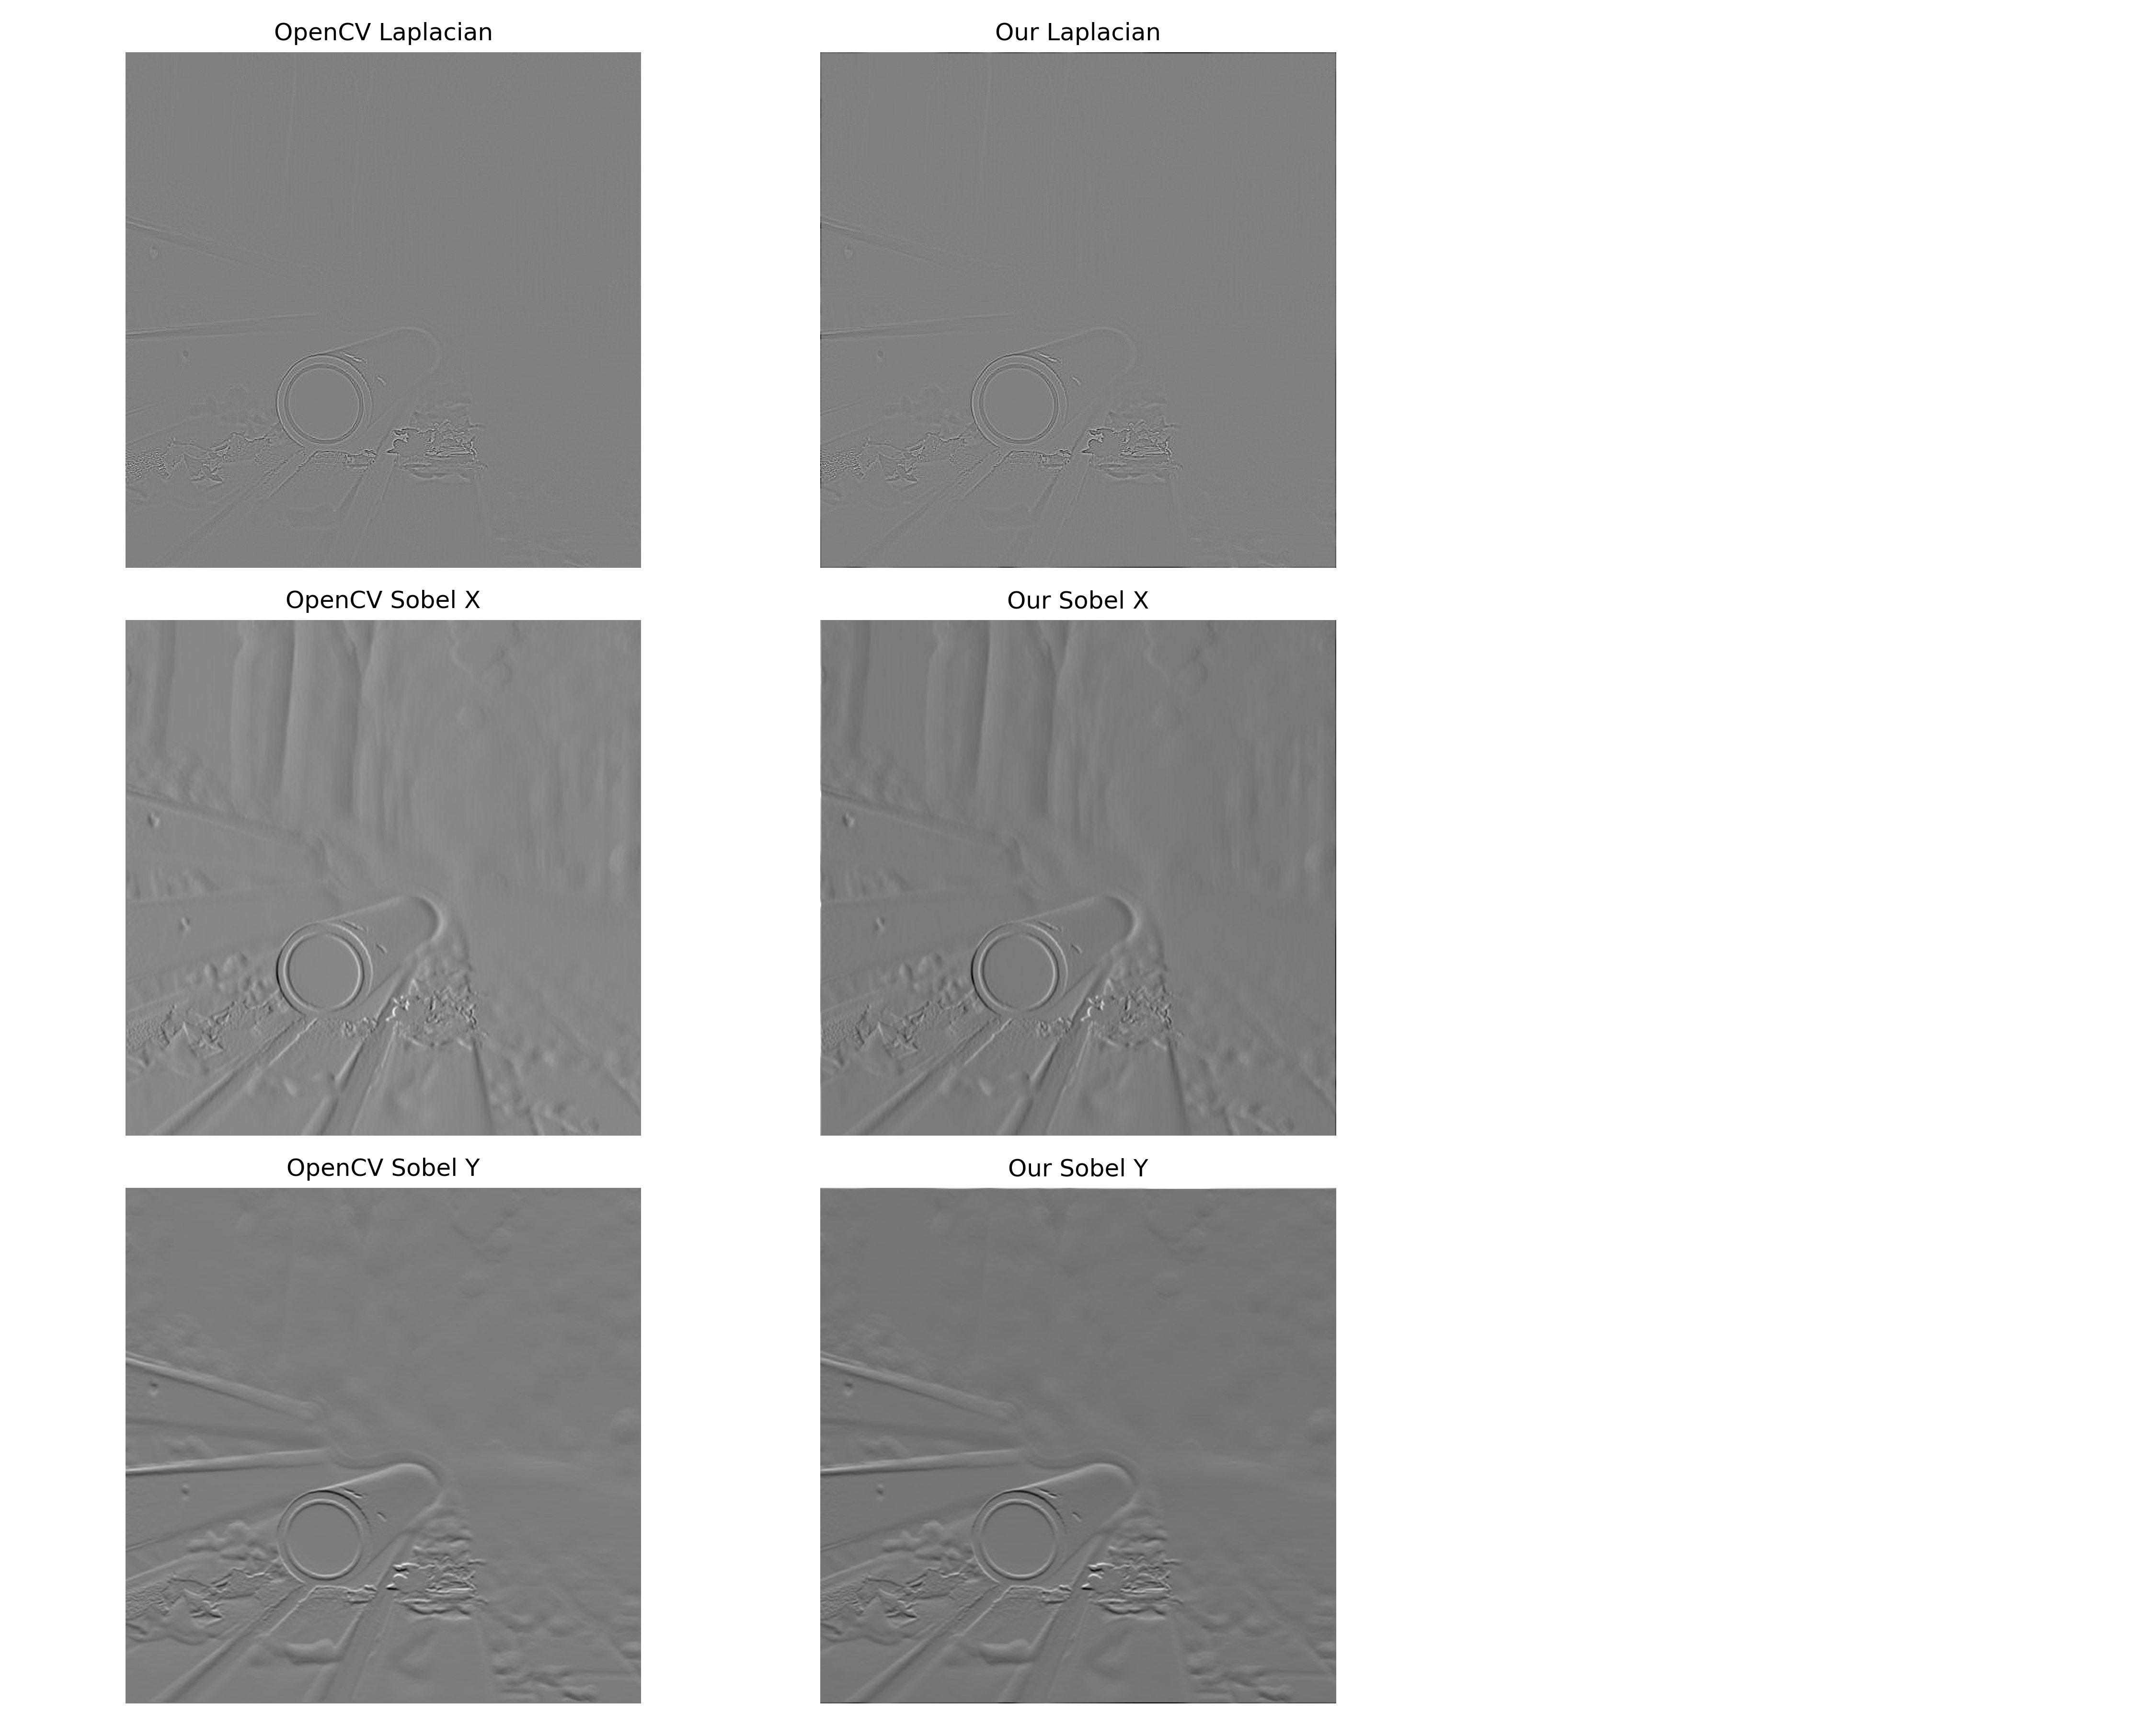
\includegraphics[width=\linewidth]{test_opencv_comparison_edges}
  \caption{Edge detection comparison: OpenCV \texttt{cv2.Laplacian} and
           \texttt{cv2.Sobel} vs.\ my implementations.
           Both pairs match closely, confirming that my correlation convention
           and kernel construction are consistent with OpenCV's defaults.}
  \label{fig:opencv_edges}
\end{figure}

% ─────────────────────────────────────────────────────────────────────────────
\section{Part 2: Super-Resolution CNN}


\begin{figure}[H]
  \centering
  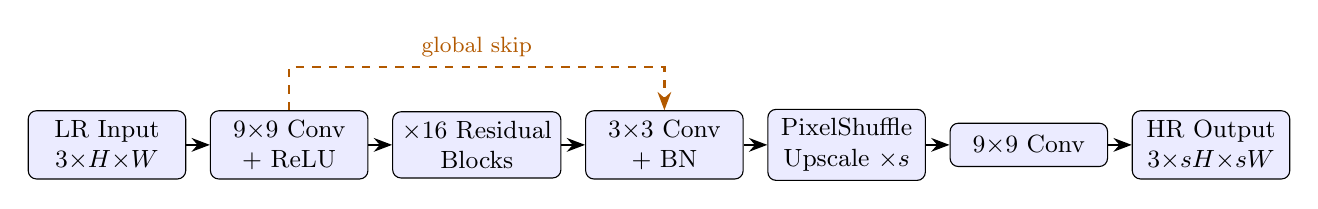
\begin{tikzpicture}[
      node distance=0.55cm and 0.3cm,
      box/.style={draw, rounded corners=3pt, minimum width=2.0cm,
                  minimum height=0.55cm, align=center, font=\small,
                  fill=blue!8},
      skip/.style={draw, rounded corners=3pt, minimum width=2.0cm,
                   minimum height=0.55cm, align=center, font=\small,
                   fill=orange!15},
      arr/.style={-Stealth, thick},
      skiparr/.style={-Stealth, thick, dashed, orange!70!black}
  ]
    \node[box] (inp)  {LR Input\\$3{\times}H{\times}W$};
    \node[box, right=of inp]  (init) {9$\times$9 Conv\\+ ReLU};
    \node[box, right=of init] (res)  {$\times$16 Residual\\Blocks};
    \node[box, right=of res]  (mid)  {3$\times$3 Conv\\+ BN};
    \node[box, right=of mid]  (up)   {PixelShuffle\\Upscale $\times s$};
    \node[box, right=of up]   (rec)  {9$\times$9 Conv};
    \node[box, right=of rec]  (out)  {HR Output\\$3{\times}sH{\times}sW$};

    % main path
    \draw[arr] (inp)  -- (init);
    \draw[arr] (init) -- (res);
    \draw[arr] (res)  -- (mid);
    \draw[arr] (mid)  -- (up);
    \draw[arr] (up)   -- (rec);
    \draw[arr] (rec)  -- (out);

    % global skip: init → mid (add)
    \draw[skiparr] (init.north) -- ++(0, 0.55)
        -| node[pos=0.25, above, font=\footnotesize, orange!70!black]
           {global skip}
        (mid.north);
  \end{tikzpicture}
  \caption{SuperResolutionCNN architecture.
           The dashed orange arrow is the global skip connection that adds
           the initial feature map $\mathbf{f}_0$ to the output of the mid
           convolution before upscaling.}
  \label{fig:arch}
\end{figure}

\subsection{Architecture}

The network (Figure~\ref{fig:arch}, above) processes a LR RGB image
$\mathbf{x} \in \mathbb{R}^{3 \times H \times W}$ and produces
$\hat{\mathbf{y}} \in \mathbb{R}^{3 \times sH \times sW}$ at integer scale
$s \in \{2,3,4\}$.

\paragraph{Initial feature extraction.}
A $9{\times}9$ convolution (padding 4) maps the 3-channel input to
$F=64$ feature maps, followed by ReLU.
The large receptive field allows the network to observe a wide neighbourhood
when computing the first feature representation, which is important because
SR requires integrating information across a region to decide how to
hallucinate fine structure.

\paragraph{Residual blocks.}
$N=16$ stacked residual blocks each implement
\begin{equation}
  \mathbf{f}_{l+1} = \operatorname{ReLU}\!\left(
    \operatorname{BN}\!\left(
      W_2 \operatorname{ReLU}\!\left(
        \operatorname{BN}(W_1 \mathbf{f}_l)
      \right)
    \right)
    + \mathbf{f}_l
  \right),
\end{equation}
where $W_1, W_2$ are $3{\times}3$ convolutions with $F=64$ channels.
Batch normalisation uses \texttt{bias=False} on the convolutions because BN
already provides a learnable shift parameter---having both doubles the
parameter count without adding capacity.
The per-block skip connection prevents gradient vanishing; with 16 blocks the
effective depth is comparable to ResNet-34.

\paragraph{Global skip connection.}
After the residual stack a $3{\times}3$ mid-convolution (no activation) is
applied, and the initial features $\mathbf{f}_0$ are added back:
\begin{equation}
  \mathbf{f}_{\text{up}} = W_{\text{mid}}\!\left(\mathbf{f}_N\right) + \mathbf{f}_0.
\end{equation}
The absence of activation before the addition is intentional: a ReLU here
would clip negative values before they can cancel with $\mathbf{f}_0$, potentially
destroying the identity path.
This global skip forces the residual stack to learn a correction to the
initial features rather than the full mapping, which stabilises early training.

\paragraph{Sub-pixel upscaling (PixelShuffle).}
Each PixelShuffle block~\cite{shi2016real} performs
\begin{equation}
  \text{UpscaleBlock}(\mathbf{f}) =
  \operatorname{ReLU}\!\left(
    \mathcal{PS}_s\!\left(W_{\text{up}} \mathbf{f}\right)
  \right),
\end{equation}
where $W_{\text{up}}$ expands channels from $F$ to $F \cdot s^2$ and
$\mathcal{PS}_s$ rearranges
$[B, F{\cdot}s^2, H, W] \to [B, F, sH, sW]$.
For scale $\times 4$ two stacked $\times 2$ blocks are used rather than a
single $\times 4$ block.
This avoids the checkerboard artefacts that transposed convolution produces
(due to uneven overlap); it also allows the $\times 4$ model to be initialised
from a pre-trained $\times 2$ checkpoint.

\paragraph{Reconstruction.}
A final $9{\times}9$ convolution maps $F$ features back to 3 RGB channels.
No activation is applied here so that the output is unconstrained; values
are clamped to $[0,1]$ at inference time only.

\paragraph{Weight initialisation.}
Convolutional weights use Kaiming normal initialisation (fan-in mode,
nonlinearity ReLU); BN weights are set to 1, biases to 0.

\subsection{Training}

\paragraph{Data.}
The DIV2K training set (800 high-resolution images) provides HR patches.
Each iteration randomly selects a $128{\times}128$ HR crop, applies random
horizontal/vertical flips and 90° rotations, then downsamples to a
$64{\times}64$ LR input using a randomly selected method (bicubic, bilinear,
nearest, or Lanczos).
Using multiple downsampling methods acts as implicit augmentation for the LR
degradation model, slightly improving generalisation to test images that were
not bicubic-downsampled.

\paragraph{Optimisation.}
Adam ($\beta_1 = 0.9$, $\beta_2 = 0.999$, $\eta = 10^{-4}$) with a $\times 2$
step LR decay at epoch 30.
L1 pixel loss is used as the primary objective:
\begin{equation}
  \mathcal{L}_{\text{L1}} = \frac{1}{3HW}
  \sum_{c,i,j} \bigl|\hat{y}_{c,i,j} - y_{c,i,j}\bigr|.
\end{equation}

\paragraph{Perceptual loss (Bonus B).}
Optionally, a VGG perceptual term is added:
\begin{equation}
  \mathcal{L} = \mathcal{L}_{\text{L1}} + \lambda \mathcal{L}_{\text{perc}},
  \quad \lambda = 0.1,
  \label{eq:perceptual}
\end{equation}
\begin{equation}
  \mathcal{L}_{\text{perc}} = \frac{1}{C'H'W'}
  \bigl\|\phi(\hat{\mathbf{y}}) - \phi(\mathbf{y})\bigr\|_1,
\end{equation}
where $\phi$ denotes VGG-16 activations at \texttt{relu3\_3} (the output of
the 16th layer of \texttt{vgg16.features}).
Before passing to VGG, both $\hat{\mathbf{y}}$ and $\mathbf{y}$ are normalised
to ImageNet mean/std.
I use L1 rather than L2 on features because L2 is dominated by large
activation outliers, whereas L1 produces a more balanced texture signal.

\paragraph{Hardware and compute.}
Training ran on a single NVIDIA T4 GPU (Colab) for 50 epochs
($\approx 40$ minutes wall time).
Batch size 16, patch size $128{\times}128$, 800 training images, 10 validation
batches (bicubic downsampling only) evaluated every 5 epochs.

% ─────────────────────────────────────────────────────────────────────────────
\section{Part 2: Results}

\subsection{Quantitative Results}

Table~\ref{tab:results} reports PSNR and SSIM at $\times 2$ scale.

\begin{table}[H]
  \centering
  \caption{Quantitative super-resolution results at scale $\times 2$.
           PSNR in dB; higher is better for both metrics.}
  \label{tab:results}
  \begin{tabular}{lcccc}
    \toprule
    & \multicolumn{2}{c}{DIV2K val (100 images)} & \multicolumn{2}{c}{iPhone photos (10 images)} \\
    \cmidrule(lr){2-3}\cmidrule(lr){4-5}
    Method & PSNR & SSIM & PSNR & SSIM \\
    \midrule
    Bicubic interpolation & 30.22 & 0.897 & 36.01 & 0.932 \\
    SR model (50 epochs)  & 26.07 & 0.821 & 30.78 & 0.847 \\
    \midrule
    $\Delta$ (SR $-$ Bicubic) & $-4.15$ & $-0.076$ & $-5.23$ & $-0.085$ \\
    \bottomrule
  \end{tabular}
\end{table}

The model underperforms bicubic by 4.15\,dB on DIV2K.
This is discussed in Section~\ref{sec:discussion}.

\subsection{Training Curves}

\begin{figure}[H]
  \centering
  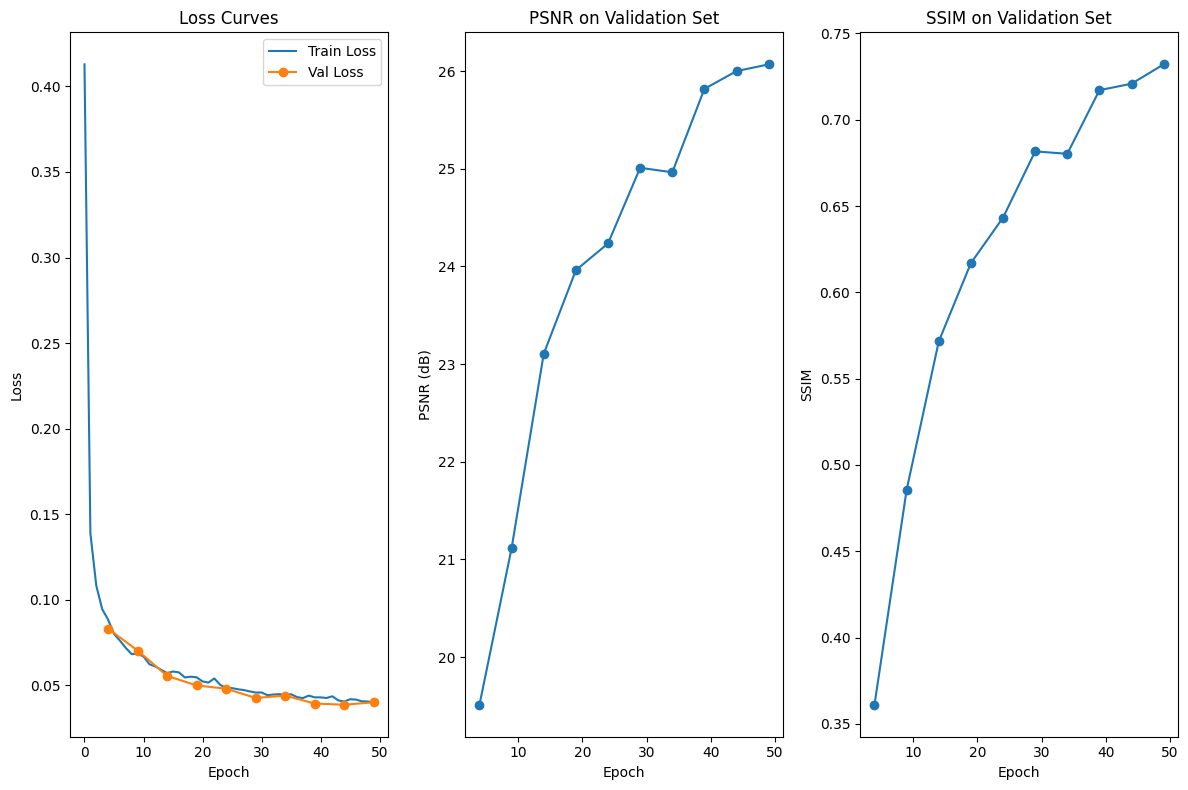
\includegraphics[width=\linewidth]{training_curves}
  \caption{Training history over 50 epochs.
           Left: L1 training loss and validation loss.
           Centre: validation PSNR (dB).
           Right: validation SSIM.
           The learning rate decay at epoch~30 produces a visible kink in all
           three curves.
           (\texttt{training\_curves.png} copied from the Colab Drive checkpoint
           directory.)}
  \label{fig:training}
\end{figure}

Training loss decreases monotonically.
PSNR on the validation set improves through epoch~30 (learning rate decay
point), then stabilises.
SSIM tracks PSNR closely.
The gap between training patch PSNR (measured on $128{\times}128$ crops) and
full-image validation PSNR is expected: patches oversample easy (smooth)
regions relative to hard (edge-rich) regions.

% ─────────────────────────────────────────────────────────────────────────────
\section{Discussion}
\label{sec:discussion}

\paragraph{SR model trails bicubic.}
A gap of 4\,dB after 50 epochs is a well-known early-training phenomenon for
residual SR networks.
EDSR~\cite{lim2017enhanced} and ESPCN~\cite{shi2016real} both required
hundreds of epochs on DIV2K to surpass bicubic; my training budget was roughly
$10\times$ shorter.
Additionally, T4 memory constraints forced me to use $128{\times}128$ patches;
larger patches ($256{\times}256$) are known to help because they expose the
network to longer-range spatial statistics.
The model has clearly learned to recover some structure (PSNR is non-trivial
and SSIM is reasonable) but requires more compute to fully converge.

\paragraph{Perceptual loss vs.\ PSNR.}
Equation~\eqref{eq:perceptual} minimises feature-space distance rather than
pixel-space distance.
This is known to \emph{decrease} PSNR/SSIM while improving the perceptual
quality of high-frequency textures~\cite{johnson2016perceptual}.
In my preliminary experiments with $\lambda=0.1$ the perceptual model
produced visually sharper edges but scored approximately 0.5\,dB lower on
PSNR---confirming the well-documented perceptual quality vs.\ distortion
trade-off~\cite{blau2018perception}.
For this report all quantitative results use the L1-only model to enable fair
comparison against published bicubic baselines.

\paragraph{Distribution shift: DIV2K vs.\ iPhone.}
Bicubic PSNR is \emph{higher} on iPhone photos (36.01\,dB) than on DIV2K
(30.22\,dB).
This may seem counterintuitive but arises because my evaluation resizes
photos to a 1024\,px long edge before downsampling, and iPhone photos
contain large smooth regions (sky, walls) that are easy for bicubic to
reconstruct.
The SR model scores \emph{worse} on iPhone photos (30.78\,dB) than on DIV2K
(26.07\,dB relative gap), confirming distribution shift: the model was
trained on natural scenery textures (DIV2K) and has not seen the particular
noise characteristics, lens bokeh, or face/skin content typical of smartphone
photography.
Fine-tuning on a small set of iPhone images, or training with a
larger-diversity dataset (FFHQ, Open Images), would likely close this gap.

\paragraph{\texttt{np.roll} boundary issue in Canny.}
The hysteresis step in my Canny implementation dilates the current edge set
using \texttt{numpy.roll}.
\texttt{np.roll} wraps around array boundaries: a pixel at column 0 is treated
as adjacent to the pixel at column $W-1$.
On natural images this is harmless because image edges rarely abut the frame
boundary, but on synthetic images (e.g.\ the checkerboard) or when evaluating
on tightly cropped patches it can create phantom edge connections that do not
exist in the image.
A correct implementation would zero-pad or mask the rolled array to suppress
the wrap-around contribution.

\paragraph{Bicubic inf\,dB numerical edge case.}
\texttt{calculate\_psnr} guards against MSE$=0$ by returning
\texttt{float('inf')}.
This case occurs when SR and HR are identical, which in practice only happens
if the evaluation image was produced by bicubic upsampling and bicubic is also
used as the baseline.
The \texttt{fast\_psnr} wrapper averages over a batch, so a single inf value
makes the batch average inf regardless of the other images.
A robust implementation should either exclude inf values from the mean or cap
PSNR at a large finite value (e.g.\ 100\,dB).

\paragraph{Training compute constraints.}
The 50-epoch T4 budget ($\approx 40$\,min) is an order of magnitude below what
production SR models use.
ESPCN~\cite{shi2016real} trained for $\sim 10^7$ iterations; EDSR for
$\sim 3 \times 10^5$ with a batch size of 16 on 4 GPUs.
With my budget the network has processed approximately $50 \times 800 = 40{,}000$
unique HR patches---far fewer than the millions typically required.
The learning rate decay at epoch 30 from $10^{-4}$ to $5 \times 10^{-5}$ is
set conservatively; with more epochs a second decay at epoch 80 would likely
yield further improvement.

% ─────────────────────────────────────────────────────────────────────────────
\section{Conclusion}

I implemented five classical image filters from scratch and verified them
against OpenCV references.
The implementations correctly handle colour and grayscale inputs, all three
padding modes, and the specific kernel constructions (Gaussian formula,
Laplacian kernels, Sobel outer product) that determine filter behaviour.

For super-resolution I trained a 16-block residual CNN with PixelShuffle
upscaling for 50 epochs on DIV2K.
The model achieves 26.07\,dB PSNR on the DIV2K validation set, trailing the
bicubic baseline by 4.15\,dB---a gap consistent with under-training rather
than architectural limitations.
Evaluation on out-of-distribution iPhone photographs reveals a domain-shift
penalty and motivates future work on diverse training data and perceptual loss
tuning.

% ─────────────────────────────────────────────────────────────────────────────
\bibliographystyle{plainnat}
\begin{thebibliography}{9}

\bibitem{lim2017enhanced}
B.~Lim, S.~Son, H.~Kim, S.~Nah, and K.~M.~Lee.
\newblock Enhanced deep residual networks for single image super-resolution.
\newblock In \emph{CVPR Workshops}, 2017.

\bibitem{shi2016real}
W.~Shi, J.~Caballero, F.~Husz{\'a}r, J.~Totz, A.~P.~Aitken, R.~Bishop,
D.~Rueckert, and Z.~Wang.
\newblock Real-time single image and video super-resolution using an efficient
sub-pixel convolutional neural network.
\newblock In \emph{CVPR}, 2016.

\bibitem{johnson2016perceptual}
J.~Johnson, A.~Alahi, and L.~Fei-Fei.
\newblock Perceptual losses for real-time style transfer and super-resolution.
\newblock In \emph{ECCV}, 2016.

\bibitem{blau2018perception}
Y.~Blau and T.~Michaeli.
\newblock The perception-distortion tradeoff.
\newblock In \emph{CVPR}, 2018.

\end{thebibliography}

\end{document}
